%% =====================================================================
%%  Supplemental Material for the PRR submission
%%  APS REVTeX 4.2, single-column [preprint] layout.
%%
%%  Reuses every supplement wrapper (and therefore every canonical
%%  derivation file under ../docs/derivations) unchanged.  Differences
%%  from the original supplement.tex:
%%    * revtex4-2 instead of article (amsthm dropped; the derivations
%%      use only a plain {theorem} environment and no {proof}).
%%    * APS-style S-prefixed numbering: Eq. (S1), Fig. S1, Table S1,
%%      Theorem S1, Section SI.  The main text picks these up
%%      automatically through xr-hyper/\externaldocument.
%%    * "Supplemental Material" (APS terminology) in the title.
%% =====================================================================
\documentclass[aps,prresearch,preprint,nofootinbib]{revtex4-2}

\usepackage{amsmath}
\usepackage{amssymb}
\usepackage{mathtools}
\usepackage{mathrsfs}
\usepackage{bm}
\usepackage{graphicx}
\usepackage{booktabs}
\usepackage{array}
\usepackage{microtype}
\usepackage[hidelinks]{hyperref}

% Shared semantic notation. Computed values are exported separately to
% paper/generated/results_macros.tex.
% Suppress engine-generated timestamps, trailer IDs, and PTEX provenance so
% SOURCE_DATE_EPOCH-controlled builds are byte reproducible.
\ifdefined\pdfinfoomitdate
  \pdfinfoomitdate=1
\fi
\ifdefined\pdftrailerid
  \pdftrailerid{}
\fi
\ifdefined\pdfsuppressptexinfo
  \pdfsuppressptexinfo=-1
\fi
\newcommand{\ZGV}{ZGV}
\newcommand{\MorseBott}{Morse--Bott}
\newcommand{\kvec}{\bm{k}}
\newcommand{\xvec}{\bm{x}}
\newcommand{\uvec}{\bm{u}}
\newcommand{\nvec}{\bm{n}}
\newcommand{\dd}{\mathop{}\!\mathrm{d}}
\newcommand{\ii}{\mathrm{i}}
\newcommand{\ee}{\mathrm{e}}
\newcommand{\order}{\mathcal{O}}
\newcommand{\abs}[1]{\left\lvert #1 \right\rvert}
\newcommand{\norm}[1]{\left\lVert #1 \right\rVert}
\DeclareMathOperator{\Hess}{Hess}
\DeclareMathOperator{\diag}{diag}
\DeclareMathOperator{\sgn}{sgn}

\newcommand{\ZGVKappa}{0.804217}
\newcommand{\ZGVOmega}{2.85176}
\newcommand{\ZGVCurvature}{1.19686}
\newcommand{\VFour}{0.0140638}
\newcommand{\SplittingSlope}{0.995817}
\newcommand{\RemainderSlope}{1.99957}
\newcommand{\EarlyDecaySlope}{-0.518693}
\newcommand{\LateDecaySlope}{-0.965731}
\newcommand{\MaxPhaseError}{1.28586\times10^{-6}}
\newcommand{\MorseMinimumCount}{4}
\newcommand{\MorseSaddleCount}{4}

% Central caption registry shared by the main paper and Supplementary Information.

\newcommand{\FigureOneCaption}{Mechanism overview on the selected branch.
\textbf{a}, Thin grey contours show the isotropic full-wave local-frequency
surface, and the solid grey curve marks the continuous ZGV ring at the exact
isotropic radius \(\kappa_0\).  \textbf{b}, Angular anomaly of the perturbation: the difference between
the anisotropic and isotropic surfaces with its mean over angle removed at
each radius.  The removed part is the angle-independent carrier shift,
which moves the ring without breaking it, so the fourfold remainder shown
here is the part that breaks it.  Troughs and crests are shaded in the
minimum and saddle colours; the computed, independently refined minima
(blue circles) and saddles (orange diamonds) fall on the troughs and
crests respectively, within the declared local annulus.  Marker shape
duplicates colour, and the panel regroups the two stored surfaces without
introducing a new computation.  \textbf{c}, Conceptual summary of the
change from a one-dimensional critical ring with generic \(t^{-1/2}\) decay to
isolated Morse points with generic \(t^{-1}\) decay; this panel is explanatory
rather than numerical, with the computed asymptotic slices tested in
Fig.~\ref{fig:decay-crossover}.  This mechanism overview does not carry the
numerical realization claim; the finite-resolution full-wave search,
Cartesian Hessians, and stability checks are reported in
Fig.~\ref{fig:morse-points}.  Wavevector components are normalized as
\(k_xh\) and \(k_yh\), frequencies as \(\Omega=\omega h/c_T\), and panels
\textbf{a} and \textbf{b} use common axes.  Source data:
\texttt{data/source\_data/figure\_01}.}

\newcommand{\FigureTwoCaption}{Independent numerical verification of the
isotropic reference.  \textbf{a}, The solid curve is the independently
discretized full-wave symmetric branch; the open orange circular symbol marks
the exact Rayleigh--Lamb reference \((\kappa_0,\Omega_0)\).  \textbf{b}, The
solid curve with circular markers is the local full-wave branch, whereas the
dashed line is the coefficient prediction
\(\Omega_0+a(\kappa-\kappa_0)^2/2\).  The positive curvature \(a\) is obtained
from exact implicit differentiation, not from a fit to the plotted samples.
\textbf{c}, Coloured marker--lines on the left axis report relative
\(\kappa_0\), \(\Omega_0\), and curvature errors together with the normalized
eigen residual, Hermitian defect, and mass-orthogonality defect; the
short-dashed line on the right axis is the relative eigengap.  \textbf{d},
Through-thickness profiles of the mass-normalized mode: solid, short-dashed,
and long-dashed curves denote \(\lvert u_x\rvert\), \(\lvert u_y\rvert\), and
\(\lvert u_z\rvert\), divided by their common global maximum.  The neutral
dotted curve is the squared-displacement proxy \(\sum_i\lvert u_i\rvert^2\),
normalized by its own maximum; it is neither a signed-parity nor a strain-energy
diagnostic.  Here \(\kappa=kh\), \(\Omega=\omega h/c_T\), and \(z/h\) is the
normalized thickness coordinate.  Source data:
\texttt{data/source\_data/figure\_02}.}

\newcommand{\FigureThreeCaption}{Full-elastic sensitivities for the declared
weak cubic family.  \textbf{a}, The solid curve is the analytic full-elastic
coefficient \(V(\theta)-V_0\), and the dashed curve is
\(V_4\cos(4\theta)\).  A common radial offset is used only to render the polar
plot, and the rings are drawn unlabelled; the outermost petal reaches
\(\lvert V_4\rvert\) in units of \(\Omega/\varepsilon\), whose value is
given in panel \textbf{c}.  \textbf{b}, Stems and circular markers show every
stored harmonic amplitude \(\lvert V_m\rvert\) on a logarithmic scale; the
\(m=4\) marker is highlighted and non-fourfold leakage is retained.
\textbf{c}, Filled circles show the stored physical shift
\(\varepsilon V_4\), while the dashed line shows \(Q_4\Delta_C\).  Their
agreement checks the perturbation convention
\(V_4=Q_4\Delta_C^{(1)}\) and
\(\Delta_C=\varepsilon\Delta_C^{(1)}\), rather than providing an independent
full-wave comparison.  \textbf{d}, Solid lines are the analytic full-elastic
\(V\) and \(B=\partial_\kappa V\); open circles and squares are independent
centered full-wave finite differences.  Agreement is quantified by the relative errors
\(\lVert V_{\rm FD}-V\rVert_2/\lVert V\rVert_2\) and
\(\lVert B_{\rm FD}-B\rVert_2/\lVert B\rVert_2\), which the build asserts
to lie below the registered tolerance.  The inset gives the
declared centered-difference step convergence of the relative \(V_4\) and
\(B\) errors.  Source data: \texttt{data/source\_data/figure\_03}.}

\newcommand{\FigureFourCaption}{Full-wave numerical realization of the local
Morse splitting with eight resolved roots.  \textbf{a}, Grey contours show the isotropic full-wave surface,
the solid grey curve marks the exact isotropic critical ring, and the two
short-dashed circles delimit the declared annulus.  \textbf{b}, Filled and
line contours show the anisotropic full-wave surface using the same levels as
panel \textbf{a}; blue circles and orange diamonds are the stored refined
minima and saddles, and the short-dashed circles again show the annular
boundaries.  \textbf{c}, Cartesian Hessian eigenvalues are ordered by
critical-point angle on a symmetric logarithmic axis.  Marker shape and colour
identify Morse class, filled and open symbols denote \(\lambda_1\) and
\(\lambda_2\), vertical bars give the declared Hessian-discrepancy estimate,
and the shaded band spans the maximum such estimate about zero.
\textbf{d}, Filled symbols joined by the solid guide line give the signed
radial error
\((\kappa_{\rm full}-\kappa_{\rm pert})/\kappa_0\); open symbols joined by the
dashed guide line give the signed frequency error
\((\Omega_{\rm full}-\Omega_{\rm pert})/\Omega_0\).  The perturbation values
are first-order predictions, and neither guide line is a fit.  All surfaces
and coordinates use the normalized \(kh\) and \(\omega h/c_T\) convention.
Source data: \texttt{data/source\_data/figure\_04}.}

\newcommand{\FigureFiveCaption}{Perturbation checks over the complete
declared weak-anisotropy sequence.  \textbf{a}, Open circles are the
full-wave minimum--saddle frequency splitting, and the dashed line is its
first-order coefficient prediction.  The reported splitting slope is an
unweighted log--log fit over every declared positive \(\lvert\varepsilon\rvert\),
not a plot-selected range; no separate fitted line is drawn.  \textbf{b}, Blue
circles and orange diamonds show the baseline-corrected full-wave radial shifts
\(q_{\min}/\varepsilon\) and \(q_{\rm sad}/\varepsilon\), while the
corresponding dashed lines are the coefficient limits
\(-B(\theta_j)/a\).  The annotated radial slope is obtained from the
uncompensated quantity \(\max(\lvert q_{\min}\rvert,\lvert q_{\rm sad}\rvert)\)
over the same complete sequence.  \textbf{c}, Markers and connecting guide
lines show the absolute full-wave minus first-order critical-frequency errors
divided by \(\varepsilon^2\) for the minimum and saddle families.  The
reported remainder slope is fitted to the maximum uncompensated error across
the two families; the connecting lines are not fits.  \textbf{d}, Circle and
diamond markers show the minimum and saddle angular orbits for opposite
perturbation signs, demonstrating exchange of the axis and diagonal roles
under \(\varepsilon\rightarrow-\varepsilon\).  Source data:
\texttt{data/source\_data/figure\_05}.}

\newcommand{\FigureSixCaption}{Two numerical asymptotic slices of the
coefficient-resolved response \(G^+\), with \(t=t_{\rm phys}c_T/h\).
\textbf{a}, Full-wave real parts and magnitudes, after removal of the shifted
carrier \(\Omega_0+\varepsilon V_0\) and uniform scaling, collapse onto
\(J_0(\tau)\), \(\tau=\varepsilon V_4t\), for the four declared uniform
transition rows.  The comparison is performed without fitted alignment.
\textbf{b}, Thin curves show the absolute complex error at all stored times;
thick segments show the uniform transition window \(t\geq1500\),
\(\lvert\tau\rvert\leq2\), including Bessel zeros.  \textbf{c}, Pale bands mark the two fitted
intervals.  The early fit
uses the raw \(\varepsilon=0.005\) magnitude, whereas the late fit uses four
complete beat-period RMS values in the fixed-anisotropy
\(\varepsilon=0.08\) row.
These are two slices, not one numerical time trajectory; the proved
growing-\(\lvert\tau\rvert\) overlap connects their coefficients and phases.
\textbf{d}, Crossover markers are first downward crossings of magnitude
\(0.9\) within a theory-centred bracket.  This is a theory-centred consistency
diagnostic; panel \textbf{a} is the primary numerical test.  \textbf{e}, At
\(\varepsilon=0.08\), the full integral and exact-Hessian Morse sum are compared
over \(1500\leq t\leq10200\); open markers denote cancellation samples with
coherence below \(0.30\).  \textbf{f}, Exact minimum and saddle frequencies
mark the critical-frequency features.  Their separation is
\(2\lvert\varepsilon V_4\rvert\) and the modulation magnitude is
\(\lvert\varepsilon V_4\rvert\).  Source data:
\texttt{data/source\_data/figure\_06}.}

\newcommand{\SupplementaryFigureOneCaption}{Polynomial-order and assembly
cross-checks for the selected isotropic branch.  \textbf{a}, Solid
marker--lines give relative errors in the exact Rayleigh--Lamb reference
\(\kappa_0\) (blue circles), \(\Omega_0\) (orange squares), and curvature
\(a\) (dark-blue diamonds) on logarithmic axes.  Each reported fine GLL order
\(p\) pairs a tracked evaluator at \(p-4\) with its independent diagnostic at
\(p\); the machine-precision plateaux need not be monotone.  \textbf{b}, The
same colours and markers show an independently reconstructed one-element
spectrum, while the coloured stars at the final order report the independent
two-element result.  \textbf{c}, At the shared final order, grey circles and
dark-blue stars compare the one- and two-element errors for all three
quantities.  The declared gates are relative \(\kappa_0\) and \(\Omega_0\)
errors below \(10^{-7}\), relative curvature error below \(10^{-4}\), eigen
residual below \(10^{-10}\), and relative eigengap greater than ten times the
larger of that residual and machine precision.  These are local discretization
and mesh-split diagnostics, not a proof for the complete spectrum.  Source
data: \texttt{data/source\_data/supplementary}.}

\newcommand{\SupplementaryFigureTwoCaption}{Quadrature, interpolation, and
phase-discrepancy convergence for the declared response window.  All panels use
the nested angular--radial grids \((N_\theta,N_q)=(16,65),(32,129),(64,257)\)
and a \((128,513)\) reference surface; solid curves with circular markers and
logarithmic ordinates show directly computed diagnostics.  \textbf{a}, Blue
circles give the RMS norm of the coarse-minus-reference demodulated complex
full-wave response divided by the reference-response RMS over the declared
time samples.  \textbf{b}, Blue circles give the maximum absolute frequency
error after periodic-angular and cubic-radial interpolation of each coarse
surface onto the reference grid.  \textbf{c}, Orange circles give the
accumulated inter-resolution phase-discrepancy estimator at the declared
maximum time, including interpolation and coarse/reference nested-order
frequency differences; the black short-dashed line is the declared acceptance
threshold of \(0.05\) rad.  The finest
quadrature error is required to be at most \(0.05\), and successive quadrature
and interpolation ratios at most one half.  These empirical estimators test
consistency across computed resolutions; they do not bound the unknown
continuum error or imply infinite-time phase accuracy.  Source data:
\texttt{data/source\_data/supplementary}.}

\newcommand{\SupplementaryFigureThreeCaption}{Local branch-tracking and
simple-eigenvalue diagnostics.  \textbf{a}, The solid blue curve with circles
is the mass-weighted modal assurance criterion relative to the \(\kappa_0\)
anchor over the declared local wavenumber window; the acceptance threshold
is \(0.99\).  \textbf{b}, The solid orange curve with diamonds is the relative
eigengap of the same tracked branch over that window.  \textbf{c}, On a
logarithmic ordinate, black circles and a solid line report the eigengap and
dark-blue squares and a solid line report the normalized eigen residual over
the polynomial-order sweep.  Acceptance requires residual below \(10^{-10}\)
and gap greater than ten times the larger of residual and machine precision.
Together these computed quantities support branch continuity and separation
only near the selected ZGV point; they neither identify the branch globally
nor certify unrelated modes.  Source data:
\texttt{data/source\_data/supplementary}.}

\newcommand{\SupplementaryFigureFourCaption}{Independent finite-difference
closure of the analytic generalized-eigenvalue sensitivities.  The horizontal
step axes in panels \textbf{a} and \textbf{b} are reversed so refinement runs
from left to right.  \textbf{a}, Blue circles and a solid line show the
centered-difference relative error in \(V_4\) versus
\(\Delta\varepsilon\).  \textbf{b}, Orange circles and a solid line show the
paired-step diagonal error in \(B\), defined as the Euclidean relative error
of the two-component vector at \(\theta=0\) and \(\pi/4\) when
\(\Delta\varepsilon=\Delta q\).  \textbf{c}, The logarithmically coloured
tensor-product heatmap reports the same vector error for every pair
\((\Delta\varepsilon,\Delta q)\); darker cells denote larger error and printed
annotations give the numerical values.  The sensitivity tolerance is \(10^{-4}\):
the final two \(V_4\) steps and the finest two-by-two \(B\) block satisfy it.
These full-wave centered differences are independent of the analytic
sensitivity formula, although they use the same full-wave eigensolver; they
are not fitted data.  Source data:
\texttt{data/source\_data/supplementary}.}

\newcommand{\SupplementaryFigureFiveCaption}{Sensitivity of the computed
response norm to the declared source and spectral window class.  Each ratio
uses the RMS of the demodulated complex full-wave response over the declared
time samples at \(\varepsilon=0.02\), normalized by the baseline
\((R/h,\sigma/k_0)=(0.5,0.15)\).  \textbf{a}, The annotated heatmap covers
three source radii and three super-Gaussian widths; the diverging colour scale
is centered on the normalized baseline value one.  \textbf{b}, Solid curves
with circular markers show the same ratios against \(R/h\), with colour
distinguishing \(\sigma/k_0\); the black horizontal line is the declared
baseline.  The separately computed widest-window boundary weight is required
to remain below the truncation gate \(5\times10^{-3}\).  This sweep supports
response-norm robustness within the displayed source--window class only.  It
does not establish source independence and is not evidence for either the
crossover exponents or the Morse theorem.  Source data:
\texttt{data/source\_data/supplementary}.}

\newcommand{\SupplementaryFigureSixCaption}{Finite-anisotropy silicon stress
test outside the weak-anisotropy theorem, for a [001] plate with
\(C_{11}=165.7\), \(C_{12}=63.9\), and \(C_{44}=79.6\,\mathrm{GPa}\)
(material source \texttt{doi:10.1107/S1600577514004962}).  \textbf{a}, Filled
blue shading and blue contour lines show the full-wave local-frequency surface
normalized as \(\Omega=\omega h/\sqrt{C_{44}/\rho}\); blue circles and orange
diamonds mark four refined minima and four saddles within the declared
annulus.  The shading is not a
separate quantitative colour scale.  \textbf{b}, Points are ordered by stored
index; orange circles and a solid line show the Cartesian Hessian eigenvalue
\(\lambda_1\), blue squares and a solid line show \(\lambda_2\), and the black
line marks zero.  Here marker identity denotes eigenvalue rather than Morse
class: both values are positive at minima and have opposite signs at saddles.
\textbf{c}, On a logarithmic axis, blue circles and a solid line give the
relative tracking gap, while orange diamonds and a solid line give the
stationarity residual \(\lVert\nabla_{\boldsymbol{k}}\Omega\rVert\); this panel
does not display the separately evaluated annular-boundary consistency check.
This is a finite-anisotropy stress test of the numerical search and local
classification only, not evidence for the weak-anisotropy theorem.  Source
data: \texttt{data/source\_data/supplementary}.}


%% Plain theorem environment (numbered continuously: Theorem S1, S2, ...)
\newtheorem{theorem}{Theorem}
\renewcommand{\thetheorem}{S\arabic{theorem}}

%% APS Supplemental Material numbering: S-prefixes throughout.
\renewcommand{\thesection}{S\Roman{section}}
\renewcommand{\theequation}{S\arabic{equation}}
\renewcommand{\thefigure}{S\arabic{figure}}
\renewcommand{\thetable}{S\arabic{table}}

\allowdisplaybreaks[2]
\setlength{\emergencystretch}{2em}

\begin{document}

\title{Supplemental Material for\\
``A Coefficient- and Phase-Resolved Bridge across Noncommuting Limits of
Lamb-Wave ZGV Splitting''}

%% ===== Authors and affiliations: FILL IN before submission =========
\author{Author One}
\email{author.one@example.edu}
\affiliation{Department of Mechanical Engineering, Example University,
City 00000, Country}

\author{Author Two}
\affiliation{Department of Mechanical Engineering, Example University,
City 00000, Country}
%% ===================================================================

%% No dated line, matching the main text.
\date[]{}

\maketitle

\tableofcontents

% Canonical source: do not duplicate or edit the derivation in this wrapper.
% Canonical derivation source for the exact isotropic ZGV critical ring.
% This file is a LaTeX fragment and is included by the Supplementary Information.

\section{Exact isotropic Rayleigh--Lamb branch and its Morse--Bott ring}
\label{sec:isotropic-rayleigh-lamb-derivation}

We derive the symmetric Rayleigh--Lamb equation from the displacement
potentials, retain the physical traction matrix before any algebraic
division, and then construct the determinant used by the numerical solver.
The plate occupies
\(
  \{(x,y,z):-h\leq z\leq h\}
\)
and is infinite in the in-plane coordinates.  Its density is \(\rho>0\),
and its isotropic stiffness is specified by the Lam\'e moduli \(\lambda\)
and \(\mu\), with
\begin{equation}
  c_L^2=\frac{\lambda+2\mu}{\rho},
  \qquad
  c_T^2=\frac{\mu}{\rho}.
  \label{eq:isotropic-wave-speeds}
\end{equation}
We use the time convention \(\exp[-\mathrm{i}\omega t]\).  Isotropy lets us
rotate any in-plane wave vector onto the \(x\) axis while deriving the scalar
equation; the two-dimensional wave-vector dependence is restored at the end.

\subsection{Helmholtz potentials and symmetric parity}

In the sagittal \((x,z)\) plane, the displacement
\(\mathbf{u}=(u_x,0,u_z)\) obeys Navier's equation
\begin{equation}
  \rho\,\partial_t^2\mathbf{u}
  = (\lambda+\mu)\nabla(\nabla\mathbin{\cdot}\mathbf{u})
    +\mu\nabla^2\mathbf{u}.
  \label{eq:navier-isotropic}
\end{equation}
Introduce a longitudinal potential \(\phi\) and a sagittal shear potential
\(\psi\) by
\begin{equation}
  \mathbf{u}
  =\nabla\phi+\nabla\mathbin{\times}(\psi\,\mathbf{e}_y),
  \qquad
  u_x=\partial_x\phi-\partial_z\psi,
  \qquad
  u_z=\partial_z\phi+\partial_x\psi.
  \label{eq:helmholtz-sagittal}
\end{equation}
The divergence of the curl term is zero and the curl of the gradient term is
zero.  Taking the divergence and the sagittal curl of
Eq.~\eqref{eq:navier-isotropic}, respectively, gives the two scalar wave
equations
\begin{equation}
  \left(\nabla^2-c_L^{-2}\partial_t^2\right)\phi=0,
  \qquad
  \left(\nabla^2-c_T^{-2}\partial_t^2\right)\psi=0.
  \label{eq:potential-wave-equations}
\end{equation}
For a factor \(\exp[\mathrm{i}(kx-\omega t)]\), define the longitudinal and
shear thickness wavenumbers on their principal complex branches by
\begin{equation}
  p^2=\frac{\omega^2}{c_L^2}-k^2,
  \qquad
  s^2=\frac{\omega^2}{c_T^2}-k^2.
  \label{eq:thickness-wavenumbers}
\end{equation}
The symmetric Lamb parity is
\begin{equation}
  u_x(x,-z)=u_x(x,z),
  \qquad
  u_z(x,-z)=-u_z(x,z).
  \label{eq:symmetric-displacement-parity}
\end{equation}
Equation~\eqref{eq:helmholtz-sagittal} therefore requires an even
longitudinal potential and an odd shear potential.  With physical potential
amplitudes \(A\) and \(B\), the complete symmetric separated ansatz is
\begin{equation}
  \phi=A\cos(pz)\,\mathrm{e}^{\mathrm{i}(kx-\omega t)},
  \qquad
  \psi=B\sin(sz)\,\mathrm{e}^{\mathrm{i}(kx-\omega t)}.
  \label{eq:symmetric-potentials}
\end{equation}
Suppressing the common exponential factor from now on, direct substitution
gives
\begin{align}
  u_x(z)
  &=\mathrm{i}kA\cos(pz)-sB\cos(sz),
  \label{eq:symmetric-ux}\\
  u_z(z)
  &=-pA\sin(pz)+\mathrm{i}kB\sin(sz).
  \label{eq:symmetric-uz}
\end{align}
The first expression is even and the second is odd, so the chosen potential
parities reproduce Eq.~\eqref{eq:symmetric-displacement-parity} explicitly.

\subsection{Face tractions and the original determinant}

For an isotropic solid,
\(
  \boldsymbol{\sigma}
  =\lambda(\nabla\mathbin{\cdot}\mathbf{u})\mathbf{I}
   +2\mu\boldsymbol{\varepsilon}
\), where
\(
  \boldsymbol{\varepsilon}
  =(\nabla\mathbf{u}+\nabla\mathbf{u}^{\mathsf T})/2
\).
The derivatives of Eqs.~\eqref{eq:symmetric-ux} and
\eqref{eq:symmetric-uz} give
\begin{align}
  \varepsilon_{xx}
  &=-k^2A\cos(pz)-\mathrm{i}ksB\cos(sz),\\
  \varepsilon_{zz}
  &=-p^2A\cos(pz)+\mathrm{i}ksB\cos(sz),\\
  2\varepsilon_{xz}
  &=-2\mathrm{i}kpA\sin(pz)+(s^2-k^2)B\sin(sz).
  \label{eq:symmetric-strains}
\end{align}
Consequently,
\begin{equation}
  \frac{\sigma_{xz}}{\mu}
  =-2\mathrm{i}kpA\sin(pz)+(s^2-k^2)B\sin(sz).
  \label{eq:shear-traction-through-thickness}
\end{equation}
For the normal stress, the shear-potential terms cancel from the dilatation,
and hence
\begin{align}
  \sigma_{zz}
  &=-\left[\lambda k^2+(\lambda+2\mu)p^2\right]
       A\cos(pz)
    +2\mathrm{i}\mu ksB\cos(sz).                    \label{eq:sigma-zz-first}\\
  \lambda k^2+(\lambda+2\mu)p^2
  &=\rho\omega^2-2\mu k^2
    =\mu\left(\frac{\omega^2}{c_T^2}-2k^2\right)
    =\mu(s^2-k^2),                                    \label{eq:normal-factor-reduction}\\
  \frac{\sigma_{zz}}{\mu}
  &=-(s^2-k^2)A\cos(pz)+2\mathrm{i}ksB\cos(sz).
  \label{eq:normal-traction-through-thickness}
\end{align}
Here Eq.~\eqref{eq:normal-factor-reduction} uses both relations in
Eq.~\eqref{eq:thickness-wavenumbers} and \(\rho c_T^2=\mu\).

Traction freedom means \(\sigma_{xz}=\sigma_{zz}=0\) on each face.  At the
upper face \(z=+h\), Eqs.~\eqref{eq:shear-traction-through-thickness} and
\eqref{eq:normal-traction-through-thickness} become
\begin{equation}
  \underbrace{\begin{pmatrix}
    -2\mathrm{i}kp\sin(ph) & (s^2-k^2)\sin(sh)\\
    -(s^2-k^2)\cos(ph) & 2\mathrm{i}ks\cos(sh)
  \end{pmatrix}}_{\displaystyle T_S(k,\omega)}
  \begin{pmatrix}A\\B\end{pmatrix}=\mathbf{0}.
  \label{eq:traction-plus}
\end{equation}
At the lower face \(z=-h\), oddness of \(\sigma_{xz}\) and evenness of
\(\sigma_{zz}\) give the separate equations
\begin{equation}
  \begin{pmatrix}
    2\mathrm{i}kp\sin(ph) & -(s^2-k^2)\sin(sh)\\
    -(s^2-k^2)\cos(ph) & 2\mathrm{i}ks\cos(sh)
  \end{pmatrix}
  \begin{pmatrix}A\\B\end{pmatrix}=\mathbf{0}.
  \label{eq:traction-minus}
\end{equation}
The first row of Eq.~\eqref{eq:traction-minus} is the negative of the first
row of Eq.~\eqref{eq:traction-plus}, while the second rows coincide.
Therefore either face supplies the same two independent scalar conditions,
and satisfaction on one face enforces satisfaction on the other for a mode
of the stated parity.

Before any amplitude rescaling, the determinant of the physical traction
matrix in Eq.~\eqref{eq:traction-plus} is
\begin{align}
  F_S(k,\omega)
  &=\det T_S                                                        \notag\\
  &=\left[-2\mathrm{i}kp\sin(ph)\right]
    \left[2\mathrm{i}ks\cos(sh)\right]
   -\left[(s^2-k^2)\sin(sh)\right]
    \left[-(s^2-k^2)\cos(ph)\right]                                \notag\\
  &=4k^2ps\cos(sh)\sin(ph)
    +(s^2-k^2)^2\sin(sh)\cos(ph).
  \label{eq:original-traction-determinant}
\end{align}
Thus \(F_S=0\) is the usual symmetric Rayleigh--Lamb equation wherever the
chosen potential basis is nonsingular.

\subsection{Desingularization and the shear cutoff}

At the shear cutoff \(s=0\), the basis function
\(B\sin(sz)\) collapses identically and both entries in the second column of
\(T_S\) vanish.  The resulting factor of \(s\) in
Eq.~\eqref{eq:original-traction-determinant} is therefore a basis
normalization zero, not a physical dispersion condition.  Define the regular
shear amplitude
\begin{equation}
  \widehat B=sB,
  \qquad
  B\sin(sz)=\widehat B\,\frac{\sin(sz)}{s}.
  \label{eq:regular-shear-amplitude}
\end{equation}
For \(s\neq0\), the physical and regular amplitude vectors are related by
\(
  (A,B)^{\mathsf T}=\operatorname{diag}(1,s^{-1})
  (A,\widehat B)^{\mathsf T}
\).  Hence the regular traction matrix is
\begin{align}
  \widetilde T_S
  &=T_S\operatorname{diag}(1,s^{-1}) \notag\\
  &=\begin{pmatrix}
    -2\mathrm{i}kp\sin(ph)
      &(s^2-k^2)\dfrac{\sin(sh)}{s}\\[6pt]
    -(s^2-k^2)\cos(ph)
      &2\mathrm{i}k\cos(sh)
  \end{pmatrix}.
  \label{eq:regular-traction-matrix}
\end{align}
Taking its determinant entry by entry gives
\begin{align}
  D_S(k,\omega)
  :=\det\widetilde T_S
  &=(s^2-k^2)^2\frac{\sin(sh)}{s}\cos(ph)
    +4k^2p\cos(sh)\sin(ph).
  \label{eq:desingularized-determinant}
\end{align}
For \(s\neq0\), Eqs.~\eqref{eq:original-traction-determinant} and
\eqref{eq:desingularized-determinant} satisfy exactly
\begin{equation}
  F_S=sD_S.
  \label{eq:original-regular-determinant-relation}
\end{equation}
They therefore have identical roots away from the shear cutoff.  The regular
matrix also defines the correct analytic continuation through that cutoff.

Indeed, the even entire function multiplying the second potential has the
Taylor series
\begin{equation}
  \frac{\sin(sh)}{s}
  =h-\frac{s^2h^3}{3!}+\frac{s^4h^5}{5!}
    -\frac{s^6h^7}{7!}+O(s^8),
  \qquad s\longrightarrow0.
  \label{eq:sine-ratio-series}
\end{equation}
Together with \(\cos(sh)=1-s^2h^2/2+O(s^4)\), this gives the finite matrix and
determinant limits
\begin{align}
  \widetilde T_S\big|_{s=0}
  &=\begin{pmatrix}
    -2\mathrm{i}kp\sin(ph)&-k^2h\\
    k^2\cos(ph)&2\mathrm{i}k
  \end{pmatrix},                                                    \label{eq:regular-matrix-s-cutoff}\\
  D_S\big|_{s=0}
  &=k^4h\cos(ph)+4k^2p\sin(ph).                                    \label{eq:regular-determinant-s-cutoff}
\end{align}
At this cutoff \(\omega=c_Tk\) and
\(
  p^2=(c_T^2/c_L^2-1)k^2
\); Eq.~\eqref{eq:regular-determinant-s-cutoff} is not identically zero.
It retains a zero only when the two regular face-traction equations are
linearly dependent, which is the physical condition.

The other square root causes no loss of analyticity: \(\cos(ph)\) and
\(p\sin(ph)\) are entire functions of \(p^2\), while
\(\cos(sh)\) and \(\sin(sh)/s\) are entire functions of \(s^2\).
Equation~\eqref{eq:thickness-wavenumbers} therefore supplies analytic
continuation into evanescent regions.  For real \(k\) and \(\omega\), the
continued determinant remains real even when \(p\) or \(s\) is purely
imaginary.

\subsection{Implicit dispersion derivatives}

Let \((k_0,\omega_0)\) be a root of \(D_S\) with
\begin{equation}
  D_{S,\omega}(k_0,\omega_0)\neq0.
  \label{eq:nonzero-frequency-derivative}
\end{equation}
The implicit-function theorem then supplies a unique smooth local branch
\(\omega=\omega(k)\) satisfying
\begin{equation}
  D_S(k,\omega(k))=0.
  \label{eq:implicit-dispersion-branch}
\end{equation}
In the following equations, every partial derivative of \(D_S\) is evaluated
at \((k,\omega(k))\).  One total derivative of
Eq.~\eqref{eq:implicit-dispersion-branch} gives
\begin{align}
  0
  &=\frac{\mathrm{d}}{\mathrm{d}k}D_S(k,\omega(k))
    =D_{S,k}+D_{S,\omega}\omega_k,                                  \label{eq:implicit-first-chain}\\
  \omega_k
  &=-\frac{D_{S,k}}{D_{S,\omega}}.                                  \label{eq:implicit-first-derivative}
\end{align}
Differentiating Eq.~\eqref{eq:implicit-first-chain} once more, including the
dependence of each partial derivative on both arguments, yields
\begin{align}
  0
  &=\frac{\mathrm{d}}{\mathrm{d}k}
    \left(D_{S,k}+D_{S,\omega}\omega_k\right)                         \notag\\
  &=\left(D_{S,kk}+D_{S,k\omega}\omega_k\right)
   +\left(D_{S,\omega k}+D_{S,\omega\omega}\omega_k\right)\omega_k
   +D_{S,\omega}\omega_{kk}                                         \notag\\
  &=D_{S,kk}+2D_{S,k\omega}\omega_k
    +D_{S,\omega\omega}\omega_k^2+D_{S,\omega}\omega_{kk},
  \label{eq:implicit-second-chain}
\end{align}
where equality of mixed derivatives was used in the last line.  Solving this
equation gives the general second derivative
\begin{equation}
  \omega_{kk}
  =-\frac{D_{S,kk}+2D_{S,k\omega}\omega_k
          +D_{S,\omega\omega}\omega_k^2}
         {D_{S,\omega}}.
  \label{eq:implicit-second-derivative}
\end{equation}
A zero-group-velocity point satisfies \(\omega_k(k_0)=0\).  Under
Eq.~\eqref{eq:nonzero-frequency-derivative}, this is equivalent to
\(D_{S,k}(k_0,\omega_0)=0\).  Substitution into
Eq.~\eqref{eq:implicit-second-derivative} leaves the radial curvature
\begin{equation}
  a:=\omega_{kk}(k_0)
  =-\left.\frac{D_{S,kk}}{D_{S,\omega}}
    \right|_{(k_0,\omega_0)}.
  \label{eq:zgv-curvature}
\end{equation}
Thus, with \(q=k-k_0\), Taylor's theorem gives
\begin{equation}
  \omega(k)=\omega_0+\frac{a}{2}q^2+O(q^3).
  \label{eq:isotropic-radial-normal-form}
\end{equation}

For the selected first symmetric branch (the \(S_1\)-ZGV branch within the
configured search window) and the nondimensional reference values
\(
  h=\rho=\mu=1
\) and \(\lambda=2\), so that \(c_T=1\) and \(c_L=2\), the independent
arbitrary-precision refinement of \(D_S=D_{S,k}=0\), seeded only by the
float-valued branch search, is
\begin{equation}
  k_0=0.8042173193715181,
  \qquad
  \omega_0=2.8517587749600901,
  \qquad
  a=1.1968627250739301>0.
  \label{eq:reference-isotropic-zgv-values}
\end{equation}
The executable check associated with this derivation differentiates
Eq.~\eqref{eq:desingularized-determinant} at arbitrary precision, verifies
\(D_S=D_{S,k}=0\), verifies \(D_{S,\omega}\neq0\), and compares all three
values in Eq.~\eqref{eq:reference-isotropic-zgv-values} with both the Task-4
solver and the generated reference artifact.  This is a separate
high-precision refinement of the same exact scalar determinant; the
independent thickness-resolved spectral cross-check is supplied by the
numerical validation rather than claimed here.

\subsection{Cartesian Hessian and the Morse--Bott ring}

Restore the two-dimensional wave vector
\(
  \mathbf{k}=(k_x,k_y)
\), and write
\begin{equation}
  r=|\mathbf{k}|=(k_x^2+k_y^2)^{1/2},
  \qquad
  \mathbf{e}_r=\frac{\mathbf{k}}{r},
  \qquad
  \mathbf{e}_\theta=(-e_{r,y},e_{r,x}).
  \label{eq:polar-wavevector-basis}
\end{equation}
For \(r>0\), isotropy makes the selected branch radial:
\(
  \omega^{(0)}(\mathbf{k})=f(r)
\), where \(f(k)=\omega(k)\) in the one-dimensional derivation above.  Since
\begin{equation}
  \partial_{k_i}r=\frac{k_i}{r},
  \qquad
  \partial_{k_j}\left(\frac{k_i}{r}\right)
  =\frac{\delta_{ij}}{r}-\frac{k_i k_j}{r^3},
  \label{eq:radial-coordinate-derivatives}
\end{equation}
the Cartesian gradient and Hessian follow component by component:
\begin{align}
  \partial_{k_i}\omega^{(0)}
  &=f'(r)\frac{k_i}{r},                                               \label{eq:radial-cartesian-gradient}\\
  \partial_{k_j}\partial_{k_i}\omega^{(0)}
  &=f''(r)\frac{k_i k_j}{r^2}
    +f'(r)\left(\frac{\delta_{ij}}{r}
                 -\frac{k_i k_j}{r^3}\right).                        \label{eq:radial-cartesian-hessian-components}
\end{align}
In dyadic form this is
\begin{equation}
  \nabla_{\mathbf{k}}^2\omega^{(0)}
  =f''(r)\,\mathbf{e}_r\mathbf{e}_r^{\mathsf T}
   +\frac{f'(r)}{r}
    \left(\mathbf{I}-\mathbf{e}_r\mathbf{e}_r^{\mathsf T}\right)
  =f''(r)\,\mathbf{e}_r\mathbf{e}_r^{\mathsf T}
   +\frac{f'(r)}{r}\,\mathbf{e}_\theta\mathbf{e}_\theta^{\mathsf T}.
  \label{eq:radial-cartesian-hessian}
\end{equation}
Consequently the orthogonal polar basis diagonalizes the full Cartesian
Hessian:
\begin{equation}
  \begin{pmatrix}\mathbf{e}_r&\mathbf{e}_\theta\end{pmatrix}^{\mathsf T}
  \nabla_{\mathbf{k}}^2\omega^{(0)}
  \begin{pmatrix}\mathbf{e}_r&\mathbf{e}_\theta\end{pmatrix}
  =\begin{pmatrix}
    f''(r)&0\\[2pt]
    0&f'(r)/r
  \end{pmatrix}.
  \label{eq:radial-hessian-diagonalization}
\end{equation}
At \(r=k_0\), the ZGV conditions \(f'(k_0)=0\) and \(f''(k_0)=a\) reduce
Eq.~\eqref{eq:radial-hessian-diagonalization} to
\begin{equation}
  \nabla_{\mathbf{k}}^2\omega^{(0)}\big|_{r=k_0}
  =a\,\mathbf{e}_r\mathbf{e}_r^{\mathsf T},
  \qquad
  \operatorname{spec}
  \left(\nabla_{\mathbf{k}}^2\omega^{(0)}\big|_{r=k_0}\right)
  =\{a,0\}.
  \label{eq:zgv-ring-hessian}
\end{equation}

We now state precisely when the rotationally generated ZGV circle is a
Morse--Bott critical manifold.  The hypotheses separate the local scalar
geometry from the spectral condition that makes a single elastic branch
well defined.

\begin{theorem}[Isotropic ZGV Morse--Bott ring]
\label{thm:morse-bott-ring}
Let a lossless homogeneous isotropic plate have a symmetric guided-wave
eigenbranch in an open annulus about \(r=k_0>0\).  Assume:
\begin{enumerate}
  \item the eigenvalue is simple throughout that annulus and is separated
        from every other Lamb and shear-horizontal eigenvalue by a uniform
        positive mass-normalized eigengap;
  \item the branch is \(C^3\) in \(\mathbf{k}\) and rotational invariance
        gives \(\omega^{(0)}(\mathbf{k})=f(|\mathbf{k}|)\);
  \item the regular determinant satisfies
        \(D_S(k_0,\omega_0)=D_{S,k}(k_0,\omega_0)=0\) and
        \(D_{S,\omega}(k_0,\omega_0)\neq0\); and
  \item the radial curvature
        \(a=-D_{S,kk}/D_{S,\omega}\) at \((k_0,\omega_0)\) is nonzero.
\end{enumerate}
Then, in a sufficiently small annular neighbourhood, the critical set of
\(\omega^{(0)}\) is exactly
\begin{equation}
  \Gamma_0=\{\mathbf{k}\in\mathbb{R}^2:|\mathbf{k}|=k_0\}.
  \label{eq:isotropic-critical-ring}
\end{equation}
Moreover, at every \(\mathbf{k}\in\Gamma_0\),
\begin{equation}
  \ker\nabla_{\mathbf{k}}^2\omega^{(0)}
  =\operatorname{span}\{\mathbf{e}_\theta\}
  =T_{\mathbf{k}}\Gamma_0,
  \qquad
  \left.\nabla_{\mathbf{k}}^2\omega^{(0)}\right|_{N_{\mathbf{k}}\Gamma_0}
  =[a].
  \label{eq:morse-bott-kernel-and-normal-form}
\end{equation}
Thus \(\Gamma_0\) is a one-dimensional nondegenerate Morse--Bott critical
manifold.  If \(a>0\), it is a radial minimum manifold; if \(a<0\), it is a
radial maximum manifold.
\end{theorem}

\paragraph{Proof.}
The nonzero value of \(D_{S,\omega}\) gives a unique local scalar branch by
the implicit-function theorem, and the simple uniformly gapped elastic
eigenvalue identifies that scalar root with one smooth physical mode.  From
Eq.~\eqref{eq:implicit-first-derivative},
\(f'(k_0)=0\), while Eq.~\eqref{eq:zgv-curvature} gives
\(f''(k_0)=a\neq0\).  Continuity of \(f''\) permits a sufficiently small
\(\delta>0\) such that \(f''(r)\) has the sign of \(a\) whenever
\(|r-k_0|<\delta\).  Equivalently, the fundamental theorem of calculus gives
\begin{equation}
  f'(r)=f'(k_0)+\int_{k_0}^{r}f''(\xi)\,\mathrm{d}\xi
       =(r-k_0)\int_0^1 f''\bigl(k_0+\tau(r-k_0)\bigr)\,\mathrm{d}\tau.
  \label{eq:local-critical-radius-factorization}
\end{equation}
The integral factor is nonzero in that interval, so \(f'(r)=0\) there if and
only if \(r=k_0\).  Equation~\eqref{eq:radial-cartesian-gradient} then proves
that the critical set in the annulus is exactly \(\Gamma_0\).

For each point on the ring,
Eq.~\eqref{eq:zgv-ring-hessian} maps \(\mathbf{e}_r\) to
\(a\mathbf{e}_r\) and maps \(\mathbf{e}_\theta\) to zero.  Since \(a\neq0\),
its kernel is precisely \(\operatorname{span}\{\mathbf{e}_\theta\}\), which
is the tangent line to the circle, while the restriction to the radial
normal line is the nonsingular one-by-one form \([a]\).  These are exactly
the critical-set and normal-nondegeneracy conditions in the definition of a
Morse--Bott function.  The sign of \(a\) supplies the final minimum/maximum
classification. \(\square\)

For the reference branch in Eq.~\eqref{eq:reference-isotropic-zgv-values},
\(a>0\), so the normal Morse index is zero.  The tangential zero eigenvalue is
not an accidental higher-order radial degeneracy: it is enforced by the
continuous rotational symmetry.  The cases \(a=0\),
\(D_{S,\omega}=0\), or a closing modal eigengap violate distinct hypotheses
of Theorem~\ref{thm:morse-bott-ring} and require a higher-order or
matrix-valued local reduction.


% Canonical source: do not duplicate or edit the derivation in this wrapper.
% Canonical derivation source for the weak-anisotropy unfolding of the ZGV ring.
% This file is a LaTeX fragment and is included by the Supplementary Information.

\section{Weak-anisotropy normal form and Morse splitting}
\label{sec:anisotropic-morse-derivation}

This section closes the coefficients of the weak-anisotropy normal form
directly from the Hermitian elastic eigenproblem.  We first derive the
eigenvalue sensitivity under arbitrary normalization.  We then specialize
it to the fixed-density plate and differentiate the mode in a fixed mass
gauge.  A separate tensor calculation shows why the registered cubic family
has only a constant and a fourfold term at first order.  Finally, a radial
implicit-function reduction and the exact Cartesian Hessian give the number
and Morse type of the split critical points.

Throughout, a dagger denotes the Hermitian adjoint and
\(\lambda=\omega^2\).  The in-plane polar basis is
\begin{equation}
  \mathbf n(\theta)=(\cos\theta,\sin\theta,0),
  \qquad
  \mathbf t(\theta)=(-\sin\theta,\cos\theta,0),
  \qquad
  \mathbf z=(0,0,1).
  \label{eq:anisotropic-polar-basis}
\end{equation}
The radial coordinate is denoted by \(k>0\), and
\(q=k-k_0\) measures distance from the isotropic ZGV circle.

\subsection{General Hermitian-pencil sensitivity}

Let a real parameter \(p\) enter a Hermitian generalized eigenproblem
\begin{equation}
  K(p)\mathbf u(p)=\lambda(p)M(p)\mathbf u(p),
  \qquad
  K(p)^\dagger=K(p),
  \qquad
  M(p)^\dagger=M(p)>0.
  \label{eq:general-hermitian-pencil}
\end{equation}
Assume that \(\lambda\) is simple and let
\begin{equation}
  N:=\mathbf u^\dagger M\mathbf u>0.
  \label{eq:arbitrary-mass-norm}
\end{equation}
No normalization has yet been imposed.  Differentiating
Eq.~\eqref{eq:general-hermitian-pencil} gives
\begin{equation}
  (K_p-\lambda_pM-\lambda M_p)\mathbf u
  +(K-\lambda M)\mathbf u_p=\mathbf0.
  \label{eq:differentiated-general-pencil}
\end{equation}
Left multiplication by \(\mathbf u^\dagger\) removes the last term because
\(\mathbf u^\dagger(K-\lambda M)=\mathbf0^\dagger\).  Therefore
\begin{equation}
  \lambda_p
  =\frac{\mathbf u^\dagger(K_p-\lambda M_p)\mathbf u}{N},
  \qquad
  \omega_p
  =\frac{\mathbf u^\dagger(K_p-\lambda M_p)\mathbf u}
         {2\omega N}.
  \label{eq:general-frequency-sensitivity}
\end{equation}
Both the numerator and denominator acquire the same factor \(|c|^2\) under
\(\mathbf u\mapsto c\mathbf u\), for any nonzero complex \(c\).  Thus
Eq.~\eqref{eq:general-frequency-sensitivity} is valid with arbitrary
normalization and is also phase invariant.  Hermiticity makes its numerator
real.

The present perturbation changes stiffness but not density.  Moreover, the
plate mass form is independent of the in-plane wave vector.  Hence the
fixed-density specialization is
\begin{align}
  M_k=M_\varepsilon=0,
  \qquad&
  \lambda_k=\frac{\mathbf u^\dagger K_k\mathbf u}{N},
  \notag\\
  \lambda_\varepsilon
  =\frac{\mathbf u^\dagger K_\varepsilon\mathbf u}{N},
  \qquad&
  V(k,\theta):=\omega_\varepsilon
  =\frac{\lambda_\varepsilon}{2\omega}.
  \label{eq:fixed-mass-first-sensitivities}
\end{align}
Here every derivative is taken on the tracked simple branch, and
\(K_\varepsilon\) is the stiffness derivative per unit \(\varepsilon\).

For completeness, the radial derivative of \(V\) can also be written before
choosing a normalization.  At fixed mass define
\begin{align}
  S_\varepsilon:=\mathbf u^\dagger K_\varepsilon\mathbf u,
  \qquad&
  (S_\varepsilon)_k
  =\mathbf u_k^\dagger K_\varepsilon\mathbf u
   +\mathbf u^\dagger K_{k\varepsilon}\mathbf u
   +\mathbf u^\dagger K_\varepsilon\mathbf u_k,
  \notag\\
  N_k=\mathbf u_k^\dagger M\mathbf u
      +\mathbf u^\dagger M\mathbf u_k.&
  \label{eq:arbitrary-normalization-radial-ingredients}
\end{align}
Applying the quotient rule to
\(V=S_\varepsilon/(2\omega N)\), and using
\(\omega_k=\lambda_k/(2\omega)\), yields
\begin{equation}
  \partial_kV
  =\frac{(S_\varepsilon)_k-S_\varepsilon N_k/N}{2\omega N}
   -\frac{S_\varepsilon\lambda_k}{4\omega^3N}.
  \label{eq:arbitrary-normalization-B}
\end{equation}
The combination in the first numerator cancels the derivative of any
\(k\)-dependent scale or phase of \(\mathbf u\).  Equation
\eqref{eq:arbitrary-normalization-B} is therefore normalization invariant,
as required by the left-hand side.

\subsection{Mass gauge, augmented solve, and the complete radial coefficient}

For computation and for a compact reduced-resolvent formula, choose the
mass-normalized eigenvector and its parallel-transport phase,
\begin{equation}
  \mathbf u^\dagger M\mathbf u=1,
  \qquad
  \mathbf u^\dagger M\mathbf u_k=0.
  \label{eq:mass-normalized-parallel-gauge}
\end{equation}
The real part of the second condition follows by differentiating the first;
the phase of \(\mathbf u\) is chosen to set its imaginary part to zero.  Put
\(A:=K-\lambda M\).  Equation
\eqref{eq:differentiated-general-pencil}, specialized to \(p=k\), together
with the gauge is equivalent to the augmented system
\begin{equation}
  \begin{pmatrix}
    K-\lambda M & M\mathbf u\\
    \mathbf u^\dagger M & 0
  \end{pmatrix}
  \begin{pmatrix}\mathbf u_k\\ \alpha\end{pmatrix}
  =
  \begin{pmatrix}
    -(K_k-\lambda_kM)\mathbf u\\ 0
  \end{pmatrix}.
  \label{eq:augmented-mode-derivative}
\end{equation}
For an exact simple eigenpair the multiplier is \(\alpha=0\).  The augmented
matrix is nonsingular: a homogeneous solution first gives
\(\alpha=0\) after left multiplication of its upper row by
\(\mathbf u^\dagger\); simplicity then gives
\(\mathbf x=c\mathbf u\), and the lower row forces \(c=0\).

Let \(\{(\lambda_n,\mathbf u_n)\}\) be a complete set of generalized
eigenpairs with
\(\mathbf u_m^\dagger M\mathbf u_n=\delta_{mn}\), and let the selected
mode have index zero.  Taking the inner product of the differentiated
equation with \(\mathbf u_n\), for \(n\ne0\), gives
\begin{align}
  (\lambda_n-\lambda)
  \mathbf u_n^\dagger M\mathbf u_k
  &=-\mathbf u_n^\dagger
       (K_k-\lambda_kM)\mathbf u                                      \notag\\
  &=-\mathbf u_n^\dagger K_k\mathbf u.
  \label{eq:mode-derivative-coefficient}
\end{align}
The gauge removes the component along \(\mathbf u\), so
\begin{equation}
  \mathbf u_k
  =\sum_{n\ne0}
    \mathbf u_n
    \frac{\mathbf u_n^\dagger K_k\mathbf u}{\lambda-\lambda_n}.
  \label{eq:mode-derivative-modal-sum}
\end{equation}
Equivalently, define the reduced resolvent
\begin{equation}
  \mathcal R_\lambda
  :=\sum_{n\ne0}
    \frac{\mathbf u_n\mathbf u_n^\dagger}{\lambda_n-\lambda}.
  \label{eq:reduced-resolvent}
\end{equation}
Then
\(
  \mathbf u_k=-\mathcal R_\lambda
  (K_k-\lambda_kM)\mathbf u
\).
The modal sum and the augmented system are two representations of the same
gauge-fixed derivative.  On a compact parameter set, a uniform positive
eigengap together with uniform coercivity and boundedness of the mass matrix
bounds \(\mathcal R_\lambda\) in the associated operator norms.  Here the
mass matrix is fixed and positive definite.  Loss of either hypothesis is
addressed below as a theorem boundary.

In the gauge \eqref{eq:mass-normalized-parallel-gauge}, differentiation of
\(\lambda_\varepsilon=\mathbf u^\dagger K_\varepsilon\mathbf u\)
gives the full mixed eigenvalue derivative
\begin{equation}
  \lambda_{k\varepsilon}
  =\mathbf u^\dagger K_{k\varepsilon}\mathbf u
   +2\operatorname{Re}
     (\mathbf u^\dagger K_\varepsilon\mathbf u_k).
  \label{eq:complete-mixed-eigenvalue-derivative}
\end{equation}
Consequently the radial coefficient in the frequency normal form is
\begin{align}
  B(\theta)
  :=\left.\partial_k\partial_\varepsilon\omega
    \right|_{(k_0,\theta,0)}
  &=\left.
    \left(
      \frac{\lambda_{k\varepsilon}}{2\omega}
      -\frac{\lambda_\varepsilon\lambda_k}{4\omega^3}
    \right)\right|_{(k_0,\theta,0)}                                  \notag\\
  &=\left.
    \left[
      \frac{\mathbf u^\dagger K_{k\varepsilon}\mathbf u}{2\omega}
      +\frac{\operatorname{Re}
        (\mathbf u^\dagger K_\varepsilon\mathbf u_k)}{\omega}
      -\frac{\lambda_\varepsilon\lambda_k}{4\omega^3}
    \right]\right|_{(k_0,\theta,0)}.
  \label{eq:complete-radial-frequency-sensitivity}
\end{align}
The three displayed contributions are, respectively, the explicit mixed
stiffness derivative, the differentiated-mode contribution, and the
frequency-denominator contribution.  At the exact isotropic ZGV point,
\(\lambda_k=2\omega\omega_k=0\), so the last contribution evaluates to
zero there.  It remains part of the general identity and is required away
from the exact ZGV radius.  In particular, \(B\) is not a fixed-mode strain
integral.

\subsection{Rotation and complete contraction of the cubic perturbation}

Let \(\{\mathbf a_1,\mathbf a_2,\mathbf a_3\}\) be the orthonormal cubic
axes.  A cubic elasticity tensor can be decomposed exactly as
\begin{align}
  C_{ijkl}
  ={}&C_{12}\delta_{ij}\delta_{kl}
   +C_{44}(\delta_{ik}\delta_{jl}+\delta_{il}\delta_{jk})
  \notag\\
  &+\Delta_C\sum_{\alpha=1}^{3}
      a_{\alpha i}a_{\alpha j}a_{\alpha k}a_{\alpha l},
  \qquad
  \Delta_C=C_{11}-C_{12}-2C_{44}.
  \label{eq:cubic-tensor-decomposition}
\end{align}
Indeed, the \(iiii\), \(iijj\), and \(ijij\) components of the right-hand
side are \(C_{12}+2C_{44}+\Delta_C=C_{11}\), \(C_{12}\), and
\(C_{44}\), respectively, and cubic symmetry generates all remaining
nonzero components.

The registered bulk-preserving family is
\begin{equation}
  C_{11}=\lambda+2\mu+\frac{2}{3}\varepsilon\delta,
  \qquad
  C_{12}=\lambda-\frac{1}{3}\varepsilon\delta,
  \qquad
  C_{44}=\mu.
  \label{eq:registered-cubic-family}
\end{equation}
It has
\begin{equation}
  C_{12}^{(1)}=-\frac{\delta}{3},
  \qquad
  C_{44}^{(1)}=0,
  \qquad
  \Delta_C^{(1)}
  :=\left.\partial_\varepsilon\Delta_C\right|_0=\delta,
  \qquad
  \Delta_C(\varepsilon)=\varepsilon\delta.
  \label{eq:cubic-family-derivatives}
\end{equation}
Thus Eq.~\eqref{eq:cubic-tensor-decomposition} gives
\begin{equation}
  C^{(1)}_{ijkl}
  =-\frac{\delta}{3}\delta_{ij}\delta_{kl}
   +\delta\sum_{\alpha=1}^{3}
      a_{\alpha i}a_{\alpha j}a_{\alpha k}a_{\alpha l}.
  \label{eq:registered-cubic-perturbation-tensor}
\end{equation}
The cubic stability inequalities reduce to
\(\mu>0\), \(2\mu+\varepsilon\delta>0\), and
\(3\lambda+2\mu>0\).  Thus, for the registered \(\delta>0\), stability
requires \(\varepsilon>-2\mu/\delta\); the weak signed interval used below is
chosen as a compact neighbourhood of zero inside this bound.  No assertion is
made for arbitrarily large negative \(\varepsilon\).

For a [001]-cut plate, take the crystallographic axes to be
\(\mathbf a_1=\mathbf e_x\),
\(\mathbf a_2=\mathbf e_y\), and
\(\mathbf a_3=\mathbf e_z\).  The rotation whose columns are
\((\mathbf n,\mathbf t,\mathbf z)\) is
\begin{equation}
  R(\theta)=
  \begin{pmatrix}
    \cos\theta&-\sin\theta&0\\
    \sin\theta& \cos\theta&0\\
    0&0&1
  \end{pmatrix},
  \qquad
  \widetilde C^{(1)}_{abcd}(\theta)
  =R_{ia}R_{jb}R_{kc}R_{ld}C^{(1)}_{ijkl}.
  \label{eq:cubic-tensor-rotation}
\end{equation}
The isotropic sagittal mode propagating along \(\mathbf n\) has displacement
\begin{equation}
  \widehat{\mathbf u}(z;\theta)
  =U(z)\mathbf n+W(z)\mathbf z,
  \label{eq:isotropic-sagittal-mode}
\end{equation}
and strain
\begin{align}
  \boldsymbol\epsilon
  ={}&E\,\mathbf n\mathbf n
   +Z\,\mathbf z\mathbf z
   +S(\mathbf n\mathbf z+\mathbf z\mathbf n),
  \notag\\
  &E=\mathrm{i}k_0U,
  \qquad
  Z=W',
  \qquad
  S=\frac{U'+\mathrm{i}k_0W}{2}.
  \label{eq:sagittal-strain-components}
\end{align}
Writing \(c=\cos\theta\) and \(s=\sin\theta\), its six independent
components in the crystal frame are
\begin{equation}
  \epsilon_{xx}=c^2E,
  \quad
  \epsilon_{yy}=s^2E,
  \quad
  \epsilon_{zz}=Z,
  \quad
  \epsilon_{xy}=csE,
  \quad
  \epsilon_{xz}=cS,
  \quad
  \epsilon_{yz}=sS.
  \label{eq:rotated-sagittal-strain}
\end{equation}

Before inserting the special family, the complete cubic strain contraction
is
\begin{align}
  \epsilon_{ij}^*C^{(1)}_{ijkl}\epsilon_{kl}
  ={}&C_{11}^{(1)}
      (|\epsilon_{xx}|^2+|\epsilon_{yy}|^2+|\epsilon_{zz}|^2)       \notag\\
    &+2C_{12}^{(1)}\operatorname{Re}
      (\epsilon_{xx}^*\epsilon_{yy}
       +\epsilon_{xx}^*\epsilon_{zz}
       +\epsilon_{yy}^*\epsilon_{zz})                              \notag\\
    &+4C_{44}^{(1)}
      (|\epsilon_{xy}|^2+|\epsilon_{xz}|^2+|\epsilon_{yz}|^2).
  \label{eq:complete-cubic-strain-contraction}
\end{align}
Every normal and shear component in
Eq.~\eqref{eq:rotated-sagittal-strain} is represented here.  The required
trigonometric products are
\begin{equation}
  c^4+s^4=\frac{3+\cos4\theta}{4},
  \qquad
  c^2s^2=\frac{1-\cos4\theta}{8}.
  \label{eq:fourfold-trigonometric-products}
\end{equation}
Substituting Eqs.~\eqref{eq:cubic-family-derivatives},
\eqref{eq:rotated-sagittal-strain}, and
\eqref{eq:fourfold-trigonometric-products} into
Eq.~\eqref{eq:complete-cubic-strain-contraction} gives, term by term,
\begin{align}
  \epsilon^*:C^{(1)}:\epsilon
  =\delta\left[
      \frac{5}{12}|E|^2
      +\frac{2}{3}|Z|^2
      -\frac{2}{3}\operatorname{Re}(E^*Z)
      +\frac{1}{4}|E|^2\cos4\theta
    \right].
  \label{eq:registered-cubic-strain-contraction}
\end{align}
The shear strain \(S\) has zero coefficient here precisely because
\(C_{44}^{(1)}=0\), not because it was excluded from the contraction.

For a mode of arbitrary mass norm
\begin{equation}
  N=\int_{-h}^{h}\rho(|U|^2+|W|^2)\,\mathrm dz,
  \label{eq:sagittal-mode-mass-norm}
\end{equation}
the first-order sensitivity is therefore
\begin{equation}
  V(\theta)=V_0+V_4\cos4\theta,
  \label{eq:first-order-cubic-angular-sensitivity}
\end{equation}
where
\begin{align}
  V_0
  &=\frac{\delta}{2\omega_0N}
    \int_{-h}^{h}\left[
      \frac{5}{12}|E|^2+\frac{2}{3}|Z|^2
      -\frac{2}{3}\operatorname{Re}(E^*Z)
    \right]\,\mathrm dz,                                           \label{eq:cubic-vzero}\\
  V_4
  &=Q_4\Delta_C^{(1)},
  \qquad
  Q_4:=\frac{1}{8\omega_0N}\int_{-h}^{h}|E|^2\,\mathrm dz
      =\frac{k_0^2}{8\omega_0N}\int_{-h}^{h}|U|^2\,\mathrm dz>0.
  \label{eq:cubic-vfour}
\end{align}
The last inequality holds for the selected finite-wavenumber Lamb mode,
whose in-plane component is nonzero.  Since
\(\Delta_C^{(1)}=\delta>0\) in the current family, it follows analytically
that \(V_4>0\).  The reference spectral evaluation gives
\(V_4=0.014063828174045103>0\) in the registered dimensionless units.
The physical angular frequency displacement is
\begin{equation}
  \varepsilon V_4
  =Q_4\Delta_C(\varepsilon),
  \label{eq:physical-cubic-angular-shift}
\end{equation}
so \(\varepsilon\) is applied exactly once.  Cubic symmetry by itself would
allow \(\cos(8\theta)\) and further multiples of four; the explicit
first-order tensor contraction proves that they are absent for this linear
perturbation family.

\subsection{Controlled normal form and radial implicit-function reduction}

We now state the local reduction with its derivative-level remainder.  The
regularity assumptions are stronger than the minimum needed for the radial
root because later stationary-phase arguments differentiate the phase and
amplitude further.

\begin{theorem}[Weak-anisotropy normal form]
\label{thm:anisotropic-normal-form}
Let the isotropic plate possess a positive-frequency ZGV circle at
\(k=k_0>0\), with radial curvature \(a\ne0\).  Assume that, in a closed
annulus about this circle and for \(|\varepsilon|\leq\varepsilon_0\), the
tracked generalized eigenvalue is simple, the mass matrix is positive
definite, and the mass-normalized eigengap obeys
\begin{equation}
  \inf_{\theta,q,\varepsilon}
  \min_{n\ne0}|\lambda_n-\lambda|=g>0.
  \label{eq:uniform-anisotropic-eigengap}
\end{equation}
Assume also that the Hermitian pencil is sufficiently smooth that the
selected real frequency branch is \(C^6\) in the local variables.  The
elastic pencil used here is analytic, so this hypothesis is automatic away
from an eigengap closure.  Then,
after reducing the annulus if necessary,
\begin{equation}
  \omega(q,\theta;\varepsilon)
  =\omega_0+\frac{a}{2}q^2
   +\varepsilon\bigl[V(\theta)+qB(\theta)\bigr]
   +R(q,\theta,\varepsilon),
  \label{eq:controlled-anisotropic-normal-form}
\end{equation}
where \(V=\partial_\varepsilon\omega(k_0,\theta;0)\),
\(B=\partial_k\partial_\varepsilon\omega(k_0,\theta;0)\), and
\begin{equation}
  R=q^3r_{30}+\varepsilon q^2r_{12}+\varepsilon^2r_{02},
  \label{eq:normal-form-remainder-factorization}
\end{equation}
with uniformly bounded periodic \(C^3\) coefficient functions.  In
particular, with \((x)_+=\max(x,0)\), every derivative used
in the two-dimensional Morse reduction satisfies
\begin{equation}
  \left|
    \partial_q^i\partial_\theta^jR(q,\theta,\varepsilon)
  \right|
  \leq C_{ij}\left(
    |q|^{3-i}
    +|\varepsilon|\,|q|^{(2-i)_+}
    +\varepsilon^2
  \right),
  \qquad 0\leq i+j\leq2.
  \label{eq:derivative-level-c2-remainder}
\end{equation}
The same bound with \(i=1\) holds after two angular derivatives, as follows
directly from Eq.~\eqref{eq:normal-form-remainder-factorization}.  There is a
unique periodic radial stationary graph
\(q=q_*(\theta,\varepsilon)\) near zero, and
\begin{equation}
  q_*(\theta,\varepsilon)
  =-\frac{\varepsilon B(\theta)}{a}
   +O_{C^2}(\varepsilon^2).
  \label{eq:radial-shift}
\end{equation}
If
\(
  W_2(\theta):=r_{02}(0,\theta,0)
  =\tfrac12\partial_\varepsilon^2
    \omega(k_0,\theta;0)
\), the frequency restricted to this graph is
\begin{equation}
  \omega_*(\theta;\varepsilon)
  :=\omega(q_*(\theta,\varepsilon),\theta;\varepsilon)
  =\omega_0+\varepsilon V(\theta)
   +\varepsilon^2\left[
      W_2(\theta)-\frac{B(\theta)^2}{2a}
    \right]
   +O_{C^2}(\varepsilon^3).
  \label{eq:reduced-angular-frequency-second-order}
\end{equation}
\end{theorem}

\paragraph{Proof.}
The uniform eigengap and simplicity make the spectral projector and the
selected eigenvalue smooth.  Taylor expansion first in \(q\) and then in
\(\varepsilon\), using
\(
  \omega_q(0,\theta;0)=0
\),
\(
  \omega_{qq}(0,\theta;0)=a
\), and isotropic independence of \(\theta\), gives
Eqs.~\eqref{eq:controlled-anisotropic-normal-form} and
\eqref{eq:normal-form-remainder-factorization}.  Applying the product rule
to the three factored terms gives
Eq.~\eqref{eq:derivative-level-c2-remainder} derivative by derivative.

Radial stationarity is the equation
\begin{equation}
  F(q,\theta,\varepsilon)
  :=\omega_q
  =aq+\varepsilon B(\theta)+R_q=0.
  \label{eq:radial-stationarity-equation}
\end{equation}
At \((q,\varepsilon)=(0,0)\), one has
\(F=0\) and \(F_q=a\ne0\).  The parameter-dependent
implicit-function theorem, applied uniformly on the compact angular circle,
gives the unique periodic graph.  It first gives \(q_*=O(\varepsilon)\).
The \(i=1\) bound in
Eq.~\eqref{eq:derivative-level-c2-remainder} then gives
\(
  R_q(q_*,\theta,\varepsilon)=O_{C^2}(\varepsilon^2)
\).  Solving Eq.~\eqref{eq:radial-stationarity-equation} for \(q_*\) proves
Eq.~\eqref{eq:radial-shift}.

At \(q_*=O(\varepsilon)\), the three parts of the remainder are
\begin{equation}
  q_*^3r_{30}=O_{C^2}(\varepsilon^3),
  \qquad
  \varepsilon q_*^2r_{12}=O_{C^2}(\varepsilon^3),
  \qquad
  \varepsilon^2r_{02}
  =\varepsilon^2W_2+O_{C^2}(\varepsilon^3).
  \label{eq:remainder-on-radial-graph}
\end{equation}
Finally,
\begin{equation}
  \frac a2q_*^2+\varepsilon q_*B
  =-\frac{\varepsilon^2B^2}{2a}
   +O_{C^2}(\varepsilon^3),
  \label{eq:radial-relaxation-energy}
\end{equation}
which proves Eq.~\eqref{eq:reduced-angular-frequency-second-order}.
\(\square\)

\subsection{Exact Cartesian Hessian and its Schur inertia}

The Morse classification must use the Cartesian Hessian, not the matrix of
uncorrected polar second partial derivatives.  For any scalar
\(f(q,\theta)\), with \(k=k_0+q>0\), direct differentiation of
\(
  \nabla_{\mathbf k}f
  =\mathbf n f_q+\mathbf t f_\theta/k
\)
gives the Cartesian Hessian in the orthonormal polar basis:
\begin{equation}
  \begin{pmatrix}\mathbf n&\mathbf t\end{pmatrix}^{\mathsf T}
  \nabla_{\mathbf k}^2f
  \begin{pmatrix}\mathbf n&\mathbf t\end{pmatrix}
  =
  \begin{pmatrix}
    f_{qq}
      &k^{-1}f_{q\theta}-k^{-2}f_\theta\\[2pt]
    k^{-1}f_{q\theta}-k^{-2}f_\theta
      &k^{-1}f_q+k^{-2}f_{\theta\theta}
  \end{pmatrix}.
  \label{eq:general-cartesian-polar-hessian}
\end{equation}
At a critical point \((q_j,\theta_j)\), both first partial derivatives
vanish, and the exact matrix is
\begin{equation}
  \mathbf H_j
  =
  \begin{pmatrix}
    \omega_{qq}
      &k_j^{-1}\omega_{q\theta}\\[2pt]
    k_j^{-1}\omega_{q\theta}
      &k_j^{-2}\omega_{\theta\theta}
  \end{pmatrix}_{(q_j,\theta_j)},
  \qquad k_j=k_0+q_j.
  \label{eq:critical-cartesian-polar-hessian}
\end{equation}

Along the radial graph, implicit differentiation gives
\begin{equation}
  q_*'=-\frac{\omega_{q\theta}}{\omega_{qq}},
  \qquad
  \omega_*'=\omega_\theta,
  \qquad
  \omega_*''
  =\omega_{\theta\theta}
   -\frac{\omega_{q\theta}^2}{\omega_{qq}}.
  \label{eq:reduced-angular-schur-derivative}
\end{equation}
If \(\omega_{qq}\ne0\), Sylvester's law of inertia applied to
Eq.~\eqref{eq:critical-cartesian-polar-hessian} gives the exact decomposition
\begin{equation}
  \operatorname{inertia}(\mathbf H_j)
  =\operatorname{inertia}(\omega_{qq})
   +\operatorname{inertia}\left(
      \frac{\omega_*''}{k_j^2}
    \right).
  \label{eq:hessian-schur-inertia}
\end{equation}
Thus the mixed derivative changes the tangential eigenvalue through the
Schur complement; it cannot be discarded before the inertia is taken.

At a critical point generated by the normal form,
Eqs.~\eqref{eq:derivative-level-c2-remainder} and
\eqref{eq:radial-shift} give
\begin{equation}
  \mathbf H_j
  =
  \begin{pmatrix}
    a+O(\varepsilon)
      &\dfrac{\varepsilon B'(\theta_j)}{k_0}+O(\varepsilon^2)\\[8pt]
    \dfrac{\varepsilon B'(\theta_j)}{k_0}+O(\varepsilon^2)
      &\dfrac{\varepsilon V''(\theta_j)}{k_0^2}
       +O(\varepsilon^2)
  \end{pmatrix}.
  \label{eq:leading-anisotropic-cartesian-hessian}
\end{equation}
Its Schur complement is
\begin{equation}
  \frac{1}{k_j^2}\left(
    \omega_{\theta\theta}
    -\frac{\omega_{q\theta}^2}{\omega_{qq}}
  \right)
  =\frac{\varepsilon V''(\theta_j)}{k_0^2}
   +O(\varepsilon^2).
  \label{eq:leading-tangential-schur-complement}
\end{equation}
For the reference branch \(a>0\), the radial inertia is positive and the
sign of \(\varepsilon V''\) determines whether the second direction is
positive or negative.

\subsection{General even harmonic and the cubic eight-point theorem}

Reciprocity gives
\(\omega(k,\theta;\varepsilon)
 =\omega(k,\theta+\pi;\varepsilon)\).
Therefore the order \(m\) of the first nonconstant angular harmonic must be
even.  A mirror axis fixes the phase origin of each allowed harmonic, but does
not by itself remove other harmonics.  We now impose the additional
pure-leading-harmonic hypothesis
\begin{equation}
  V(\theta)=V_0+V_m\cos[m(\theta-\theta_0)],
  \qquad V_m\ne0.
  \label{eq:pure-general-even-harmonic}
\end{equation}
Its derivative has the \(2m\) simple zeros
\begin{equation}
  \theta_j^{(0)}=\theta_0+\frac{j\pi}{m},
  \qquad j=0,\ldots,2m-1,
  \label{eq:pure-harmonic-angular-roots}
\end{equation}
and
\begin{equation}
  V''(\theta_j^{(0)})
  =-m^2V_m(-1)^j.
  \label{eq:pure-harmonic-angular-curvature}
\end{equation}
Since
\(
  \omega_*'=\varepsilon V'+O_{C^1}(\varepsilon^2)
\), the ordinary implicit-function theorem at each simple zero gives
\begin{equation}
  \theta_j=\theta_0+\frac{j\pi}{m}+O(\varepsilon),
  \qquad
  k_j=k_0-\frac{\varepsilon B(\theta_j)}{a}
       +O(\varepsilon^2).
  \label{eq:general-harmonic-critical-locations}
\end{equation}
For \(a>0\), Eq.~\eqref{eq:leading-tangential-schur-complement} shows that
the points alternate between \(m\) minima and \(m\) saddles.  Reversing the
sign of \(\varepsilon V_m\) leaves the leading angular locations fixed and
exchanges their roles.  Their leading frequencies are
\begin{equation}
  \omega_j
  =\omega_0+\varepsilon[V_0+V_m(-1)^j]
   +O(\varepsilon^2),
  \qquad
  \Delta\omega_{\mathrm{ms}}
  =2|\varepsilon V_m|+O(\varepsilon^2).
  \label{eq:general-harmonic-frequency-splitting}
\end{equation}
The gradient index is \(+1\) at each minimum and \(-1\) at each saddle, so
the algebraic index sum is
\begin{equation}
  m(+1)+m(-1)=0.
  \label{eq:general-harmonic-index-sum}
\end{equation}

A fixed higher harmonic must be distinguished from the
\(O(\varepsilon)\) correction to the roots above.  Suppose instead that
\begin{equation}
  V(\theta)=V_0+V_m\cos[m(\theta-\theta_0)]
             +\mathcal H(\theta).
  \label{eq:leading-harmonic-plus-remainder}
\end{equation}
There is a constant \(c_m>0\) such that the dominance condition
\begin{equation}
  \lVert\mathcal H\rVert_{C^2}
  <c_m|V_m|
  \label{eq:higher-harmonic-dominance}
\end{equation}
preserves the \(2m\) simple zeros and their alternating curvatures.  Their
locations obey the separate estimate
\begin{equation}
  \theta_j
  =\theta_0+\frac{j\pi}{m}
   +O\left(
      \frac{\lVert\mathcal H\rVert_{C^1}}{|V_m|}
    \right)
   +O(\varepsilon).
  \label{eq:higher-harmonic-root-shift}
\end{equation}
Without a bound such as Eq.~\eqref{eq:higher-harmonic-dominance}, point-group
symmetry alone does not fix the number of angular critical points.

\begin{theorem}[Cubic Morse splitting]
\label{thm:cubic-morse-splitting}
Assume the hypotheses of Theorem~\ref{thm:anisotropic-normal-form}, take the
reference radial curvature \(a>0\), and use the [001] cubic family
\eqref{eq:registered-cubic-family} with \(\delta>0\).  Then, for every
sufficiently small nonzero \(\varepsilon\), a thin annular neighbourhood of
the isotropic ZGV circle contains exactly eight critical points of the
tracked branch.  They satisfy
\begin{equation}
  \theta_j=\frac{j\pi}{4}+O(\varepsilon),
  \qquad
  k_j=k_0-\frac{\varepsilon B(\theta_j)}{a}
       +O(\varepsilon^2),
  \qquad j=0,\ldots,7.
  \label{eq:cubic-eight-critical-points}
\end{equation}
Four are Morse minima and four are Morse saddles.  For
\(\varepsilon>0\), the odd \(j\) are minima and the even \(j\) are saddles;
for \(\varepsilon<0\), these roles reverse.  The two critical-frequency
families are separated by
\begin{equation}
  \Delta\omega_{\mathrm{ms}}
  =2|\varepsilon V_4|+O(\varepsilon^2),
  \qquad V_4=Q_4\delta>0,
  \label{eq:cubic-minimum-saddle-separation}
\end{equation}
and their total gradient index is zero.
\end{theorem}

\paragraph{Proof.}
Equations~\eqref{eq:registered-cubic-strain-contraction}--
\eqref{eq:cubic-vfour} prove, rather than infer from symmetry, that the
first-order angular sensitivity is the pure harmonic
\(V_0+V_4\cos4\theta\) and that \(V_4>0\).  Set \(m=4\) and
\(\theta_0=0\) in
Eqs.~\eqref{eq:pure-harmonic-angular-roots}--
\eqref{eq:general-harmonic-critical-locations}.  This gives eight points.
At their leading locations,
\begin{equation}
  \varepsilon V''(\theta_j)
  =-16\varepsilon V_4(-1)^j+O(\varepsilon^2).
  \label{eq:cubic-tangential-curvature-sign}
\end{equation}
The radial Schur pivot is positive, while the second pivot has the sign in
Eq.~\eqref{eq:cubic-tangential-curvature-sign}.  The stated minimum--saddle
classification and its reversal follow.  Equation
\eqref{eq:general-harmonic-frequency-splitting} supplies the separation, and
Eq.~\eqref{eq:general-harmonic-index-sum} supplies the index sum.
To prove that the count is exact, choose disjoint angular neighbourhoods of
the eight simple zeros of \(V'\).  On their compact complement,
\(\lvert V'\rvert\) has a positive lower bound.  After division by the
nonzero \(\varepsilon\), the \(O_{C^1}(\varepsilon)\) correction in
\(\omega_*'/\varepsilon\) cannot create a zero there when
\(\lvert\varepsilon\rvert\) is sufficiently small.  The radial graph is
unique at every angle by Theorem~\ref{thm:anisotropic-normal-form}; hence no
additional critical point exists in the reduced annulus.
\(\square\)

\subsection{Exceptional cases and theorem boundaries}

The condition \(V_m\ne0\) is substantive.  If a nominal coefficient such
as \(V_4\) vanishes, the following cases must be distinguished.
\begin{enumerate}
  \item If a higher harmonic \(V_\ell\cos(\ell\theta)\), with even
        \(\ell>m\), is the first nonzero nonconstant term at order
        \(\varepsilon\), the preceding calculation applies with
        \(m\) replaced by \(\ell\).
  \item If the whole first-order sensitivity is angularly constant, the
        second order reduced coefficient is
        \begin{equation}
          V_2^{\mathrm{eff}}(\theta)
          :=W_2(\theta)-\frac{B(\theta)^2}{2a}.
          \label{eq:effective-second-order-angular-potential}
        \end{equation}
        A nonzero nondegenerate harmonic of
        \(V_2^{\mathrm{eff}}\) splits the ring with tangential curvature of
        order \(\varepsilon^2\), not order \(\varepsilon\).
  \item If two or more harmonics compete at the same first nonzero order,
        the critical-point count is the zero count of their full derivative;
        it is not determined by one nominal order.  If at a root both
        \(V'=0\) and \(V''=0\), the point is degenerate and the Morse
        conclusion does not apply until the next local term is resolved.
\end{enumerate}

Two independent spectral boundaries are equally important.  If \(a=0\),
then \(F_q(0,\theta,0)=0\), the radial implicit-function argument fails,
and the balance between anisotropy and the first nonzero higher radial term
has a different scaling.  If the eigengap \(g\) closes, the reduced
resolvent becomes unbounded and a scalar tracked branch is not smooth; a
matrix-valued degenerate perturbation problem is then required.  The cases
\(k_0=0\) and \(\omega_0=0\) are also outside the present polar-ring and
positive-square-root formulation, respectively.

\subsection{Conversion to the dimensionless computational convention}

The code uses
\begin{equation}
  \kappa=kh,
  \qquad
  \Omega=\frac{\omega h}{c_T},
  \qquad
  c_T=\sqrt{\frac{\mu}{\rho}},
  \qquad
  q_\kappa=\kappa-\kappa_0=hq.
  \label{eq:anisotropic-nondimensional-variables}
\end{equation}
Writing subscripts \(\omega\) and \(\Omega\) for coefficients in the
dimensional and dimensionless frequency normal forms, the chain rule gives
\begin{equation}
  V_\Omega=\frac{h}{c_T}V_\omega,
  \qquad
  B_\Omega=\frac{1}{c_T}B_\omega,
  \qquad
  a_\Omega=\frac{1}{hc_T}a_\omega.
  \label{eq:anisotropic-coefficient-conversion}
\end{equation}
Hence
\begin{equation}
  q_{\kappa,*}
  =-\frac{\varepsilon B_\Omega}{a_\Omega}
   +O(\varepsilon^2)
  =h\left[-\frac{\varepsilon B_\omega}{a_\omega}
   +O(\varepsilon^2)\right],
  \label{eq:dimensionless-radial-shift}
\end{equation}
which is exactly the dimensional location multiplied by \(h\).  If the
dimensional invariant \(\Delta_C^{(1)}\) is retained, then
\(Q_{4,\Omega}=(h/c_T)Q_{4,\omega}\).  If stiffness is additionally divided
by \(\mu\), the corresponding coefficient absorbs the factor \(\mu\).
For the registered reference values
\(h=\rho=\mu=1\), one has \(c_T=1\), so the numerical and dimensional
coefficient values coincide in the chosen units.


% Canonical source: do not duplicate or edit the derivation in this wrapper.
% Canonical derivation source for the Green-function decay crossover.
% This file is a LaTeX fragment and is included by the Supplementary Information.

\section{Bessel--Morse asymptotics of the Green response}
\label{sec:green-function-asymptotics}

We derive the time-domain response of the ZGV branch with every Fourier,
modal, and stationary-phase constant retained.  The object propagated below
is the positive-frequency complex response.  It is not doubled.  The
physical real response is reconstructed only after the branch integral has
been evaluated.  This distinction fixes a factor of two that is otherwise
easy to hide in a loosely defined analytic signal.

Throughout this section \(a>0\), \(k_0>0\), and the time dependence of a
positive-frequency mode is \(\exp(-\mathrm{i}\omega t)\).  The hypotheses
on branch simplicity, eigengap, and smoothness are those of
Theorem~\ref{thm:anisotropic-normal-form}.  All asymptotic statements concern
the selected positive-frequency branch in a fixed annular spectral window;
contributions from other branches are separate terms in the complete Green
function.

\subsection{Fourier convention and normalization-invariant branch projection}

For an in-plane field, use the transform pair
\begin{equation}
  \widehat{\mathbf u}(\mathbf k,z,t)
  =\int_{\mathbb R^2}\mathbf u(\mathbf x,z,t)
    \mathrm e^{-\mathrm i\mathbf k\cdot\mathbf x}\,\mathrm d^2\mathbf x,
  \qquad
  \mathbf u(\mathbf x,z,t)
  =\mathscr F_2\int_{\mathbb R^2}
    \widehat{\mathbf u}(\mathbf k,z,t)
    \mathrm e^{\mathrm i\mathbf k\cdot\mathbf x}\,\mathrm d^2\mathbf k,
  \qquad
  \mathscr F_2=(2\pi)^{-2}.
  \label{eq:green-fourier-convention}
\end{equation}
At fixed \(\mathbf k\), let the thickness-discretized or weak-form dynamics
under an impulsive generalized load be
\begin{equation}
  M\ddot{\mathbf U}+K\mathbf U
  =\mathbf f\,\delta(t),
  \qquad
  K\mathbf u=\omega^2M\mathbf u,
  \qquad
  N:=\mathbf u^\dagger M\mathbf u>0.
  \label{eq:impulsive-hermitian-dynamics}
\end{equation}
The vector \(\mathbf f=\mathbf f(\mathbf k)\) includes the through-thickness
source functional, and a linear detector is written
\(D[\mathbf U]=\mathbf d^\dagger\mathbf U\).  Projecting
Eq.~\eqref{eq:impulsive-hermitian-dynamics} onto a simple mode gives
\begin{equation}
  \ddot q+\omega^2q
  =\frac{\mathbf u^\dagger\mathbf f}{N}\,\delta(t),
  \qquad
  q(t)=H(t)\frac{\mathbf u^\dagger\mathbf f}{\omega N}\sin(\omega t).
  \label{eq:projected-impulse-oscillator}
\end{equation}
Because
\begin{equation}
  \frac{\sin(\omega t)}{\omega}
  =2\operatorname{Re}\left[
      \frac{\mathrm i}{2\omega}\mathrm e^{-\mathrm i\omega t}
    \right],
  \label{eq:positive-frequency-oscillator-split}
\end{equation}
the undoubled coefficient of the positive-frequency exponential in the
detected response is
\begin{equation}
  \mathcal P(\mathbf k)
  :=\frac{\mathrm i}{2\omega}
    \frac{(\mathbf d^\dagger\mathbf u)
          (\mathbf u^\dagger\mathbf f)}
         {\mathbf u^\dagger M\mathbf u}.
  \label{eq:source-mode-detector-amplitude}
\end{equation}
This source--mode--detector amplitude is invariant under an arbitrary
nonzero complex normalization \(\mathbf u\mapsto c(\mathbf k)\mathbf u\):
the numerator and denominator both acquire \(|c|^2\), including when the
scale and phase depend on \(\mathbf k\).  Thus no mass-normalization
convention enters the observable amplitude.

In the mass-normalized, colocated top-face normal channel,
\(\mathbf d=\mathbf f=\mathbf e_z(h)\) and
\(\mathbf u^\dagger M\mathbf u=1\).  The general projection then reduces to
the phase-invariant overlap used by the numerical implementation,
\begin{equation}
  \mathcal P_n(\mathbf k)
  =\frac{\mathrm i}{2\omega_n}
    \left|u_{n,z}(h;\mathbf k)\right|^2.
  \label{eq:normal-impulse-overlap}
\end{equation}

Let \(G^{+}(t)\) denote the inverse Fourier integral made from the coefficient
in Eq.~\eqref{eq:source-mode-detector-amplitude}.  For a real load and
a real detector, the negative-frequency term is its complex conjugate after
the reciprocal wave-vector partner is included.  Consequently
\begin{equation}
  G_{\mathrm{phys}}(t)
  =G^{+}(t)+G^{+}(t)^*
  =2\operatorname{Re}G^{+}(t).
  \label{eq:physical-real-reconstruction}
\end{equation}
Equation~\eqref{eq:physical-real-reconstruction}, not an extra factor inside
\(G^{+}\), defines the physical real response.  Every theorem below is first
stated for \(G^{+}\), and the physical result follows from this equation.

For reference, a normalized circular Gaussian source of radius \(r_s\),
\begin{equation}
  s(\mathbf x)=\frac{1}{\pi r_s^2}
    \exp\left(-\frac{|\mathbf x|^2}{r_s^2}\right),
  \qquad
  \widehat s(k)=\exp\left[-\left(\frac{r_sk}{2}\right)^2\right],
  \label{eq:gaussian-source-transform}
\end{equation}
multiplies \(\mathcal P\) by \(\widehat s(k)\).  The numerical local-branch
window is the smooth super-Gaussian multiplied by the compact taper used by
the direct numerical integral,
\begin{equation}
  \chi_{\sigma_q}(q)=\exp[-(q/\sigma_q)^8]b_{\sigma_q}(q),
  \qquad q=k-k_0,
  \label{eq:green-super-gaussian-window}
\end{equation}
although an ordinary Gaussian window
\(\exp[-q^2/(2\sigma_q^2)]\) gives the same leading asymptotics.  Only
smoothness, localization inside the annulus, and a nonzero value at the
stationary set are used in the proof.  Here \(b_{\sigma_q}=1\) on
\(|q|\leq1.25\sigma_q\), \(b_{\sigma_q}=0\) on
\(|q|\geq1.5\sigma_q\), and the intervening strip uses the standard flat
step constructed from \(\exp(-1/x)\).  Hence \(b_{\sigma_q}\) is
\(C^\infty\), all endpoint derivatives vanish, every local coefficient below
is unchanged, and the numerical integral satisfies the same no-endpoint
hypothesis as the theorem.

Define the complete projected amplitude, excluding the Fourier measure and
the polar Jacobian, by
\begin{equation}
  \mathcal A(q,\theta;\varepsilon)
  :=\chi_{\sigma_q}(q)
    \exp\left[-\left(\frac{r_s(k_0+q)}{2}\right)^2\right]
    \frac{\mathrm i}{2\omega}
    \frac{(\mathbf d^\dagger\mathbf u)
          (\mathbf u^\dagger\mathbf f_z)}
         {\mathbf u^\dagger M\mathbf u}.
  \label{eq:complete-green-amplitude}
\end{equation}
Here \(\mathbf f_z\) is the unit through-thickness source functional; any
additional calibrated source strength can be included multiplicatively.
For the colocated axisymmetric normal channel in the isotropic plate,
\begin{equation}
  \mathcal A(0,\theta;0)=A_0,
  \qquad A_0\ne0.
  \label{eq:canonical-nonnodal-amplitude}
\end{equation}
In particular, \(A_0\) does not contain \(k_0\), \(\mathscr F_2\), or the
angular factor \(2\pi\).

\subsection{Local polar integral and radial stationary phase}

Let \(0<\eta<k_0\) be small enough that the selected branch remains simple
on \(|q|\leq\eta\), and let the window vanish smoothly before the annular
boundary if a compact cutoff is needed.  The exact local
positive-frequency complex response is
\begin{equation}
  G^{+}(t;\varepsilon)
  =\mathscr F_2
    \int_0^{2\pi}\!\int_{-\eta}^{\eta}
    \mathcal A(q,\theta;\varepsilon)
    \exp[-\mathrm it\omega(q,\theta;\varepsilon)]
    (k_0+q)\,\mathrm dq\,\mathrm d\theta.
  \label{eq:branch-projected-response}
\end{equation}
This displays the complete Fourier/polar measure
\((2\pi)^{-2}(k_0+q)\,\mathrm dq\,\mathrm d\theta\).

For sufficiently small \(|\varepsilon|\),
Theorem~\ref{thm:anisotropic-normal-form} supplies the unique radial
stationary graph \(q=q_*(\theta,\varepsilon)\).  Uniform one-dimensional
stationary phase in \(q\), with the angular variable treated as a compact
parameter, gives
\begin{align}
  G^{+}(t;\varepsilon)
  ={}&\mathscr F_2\,
    \mathrm e^{-\mathrm i\pi/4}
    \left(\frac{2\pi}{t}\right)^{1/2}
    \int_0^{2\pi}
    \frac{(k_0+q_*)\mathcal A(q_*,\theta;\varepsilon)}
         {\sqrt{\omega_{qq}(q_*,\theta;\varepsilon)}}
    \mathrm e^{-\mathrm it\omega_*(\theta;\varepsilon)}
    \,\mathrm d\theta
    +O(t^{-3/2}),
  \label{eq:radial-stationary-reduction}\\
  \omega_*(\theta;\varepsilon)
  ={}&\omega_0+\varepsilon V(\theta)
    +\varepsilon^2W_2^{\mathrm{eff}}(\theta)
    +O_{C^2}(\varepsilon^3),                                      \notag\\
  W_2^{\mathrm{eff}}(\theta)
  :={}&W_2(\theta)-\frac{B(\theta)^2}{2a}.
  \label{eq:effective-second-order-green-phase}
\end{align}
The last line is exactly the radial-relaxation correction derived in
Eq.~\eqref{eq:reduced-angular-frequency-second-order}.  Keeping \(W_2\)
but dropping \(-B^2/(2a)\) would give an incorrect second-order phase and,
therefore, an incorrect overlap window.

The radial onset time follows by requiring the stationary width
\((at)^{-1/2}\) to be small compared with the window width \(\sigma_q\):
\begin{equation}
  t_{\mathrm{rad}}\asymp\frac{1}{a\sigma_q^2}.
  \label{eq:radial-stationary-onset-time}
\end{equation}
The Fresnel phase in Eq.~\eqref{eq:radial-stationary-reduction} follows from
the exact continuation
\begin{equation}
  \int_{-\infty}^{\infty}
    \exp\left(-\frac{\mathrm i}{2}atq^2\right)\,\mathrm dq
  =\mathrm e^{-\mathrm i\pi/4}
    \sqrt{\frac{2\pi}{at}},
  \qquad a>0,\quad t>0,
  \label{eq:radial-fresnel-factor}
\end{equation}
where the oscillatory integral is defined by Gaussian continuation:
\begin{equation}
  \lim_{\eta\downarrow0}
  \int_{-\infty}^{\infty}
    \exp\left[-\left(\eta+\frac{\mathrm i}{2}at\right)q^2\right]
    \,\mathrm dq
  =\mathrm e^{-\mathrm i\pi/4}\sqrt{\frac{2\pi}{at}}.
  \label{eq:regularized-radial-fresnel-factor}
\end{equation}

\subsection{The joint transition limit and its exact Bessel kernel}

For the [001] cubic family,
\(V(\theta)=V_0+V_4\cos4\theta\), with \(V_4\) the sensitivity coefficient
and \(\varepsilon V_4\) the physical frequency shift.  Introduce
\begin{equation}
  \tau:=\varepsilon V_4t.
  \label{eq:green-transition-variable}
\end{equation}
The sign of \(\tau\) is retained; the resulting \(J_0\) kernel is even.

\begin{theorem}[Uniform Bessel crossover of the ZGV ring]
\label{thm:uniform-bessel-crossover}
Assume that the exact phase is \(C^6\), the amplitude is \(C^4\), the
radial curvature satisfies \(a>0\), \(V_4\ne0\), and
Eq.~\eqref{eq:canonical-nonnodal-amplitude} holds.  In the joint limit
\begin{equation}
  t\longrightarrow\infty,
  \qquad
  \varepsilon\longrightarrow0,
  \qquad
  \tau=\varepsilon V_4t\in K,
  \label{eq:distinguished-joint-limit}
\end{equation}
where \(K\subset\mathbb R\) is any fixed compact set,
\begin{equation}
  G^{+}(t;\varepsilon)
  =\mathcal C\,
    \mathrm e^{-\mathrm i(\omega_0+\varepsilon V_0)t}
    t^{-1/2}J_0(\varepsilon V_4t)
    +o(t^{-1/2}),
  \label{eq:uniform-response}
\end{equation}
uniformly for \(\tau\in K\), with the fully determined constant
\begin{equation}
  \mathcal C
  =\mathscr F_2(2\pi)k_0A_0
    \mathrm e^{-\mathrm i\pi/4}
    \sqrt{\frac{2\pi}{a}}.
  \label{eq:uniform-response-prefactor}
\end{equation}
No amplitude, phase, carrier-frequency correction, or time shift is fitted
in Eqs.~\eqref{eq:uniform-response}--\eqref{eq:uniform-response-prefactor}.
The corresponding physical real response is
\(G_{\mathrm{phys}}=2\operatorname{Re}G^{+}\).
\end{theorem}

\paragraph{Proof.}
Under Eq.~\eqref{eq:distinguished-joint-limit}, one has
\(\varepsilon=O(t^{-1})\).  Equations~\eqref{eq:radial-shift} and
\eqref{eq:effective-second-order-green-phase} therefore imply, uniformly in
\(\theta\),
\begin{align}
  q_*&=O(t^{-1}),
  &t\varepsilon^2W_2^{\mathrm{eff}}&=O(t^{-1}),
  &tO(\varepsilon^3)&=O(t^{-2}),                                    \notag\\
  \frac{(k_0+q_*)\mathcal A(q_*,\theta;\varepsilon)}
       {\sqrt{\omega_{qq}(q_*,\theta;\varepsilon)}}
  &=\frac{k_0A_0}{\sqrt a}+O(t^{-1}).
  \label{eq:joint-limit-radial-estimates}
\end{align}
Substitution into Eq.~\eqref{eq:radial-stationary-reduction} leaves the
angular identity
\begin{align}
  \int_0^{2\pi}\mathrm e^{-\mathrm i\tau\cos4\theta}\,\mathrm d\theta
  &=4\int_0^{\pi/2}\mathrm e^{-\mathrm i\tau\cos4\theta}\,\mathrm d\theta
    =\int_0^{2\pi}\mathrm e^{-\mathrm i\tau\cos\phi}\,\mathrm d\phi
    =2\pi J_0(\tau).
  \label{eq:angular-bessel-identity}
\end{align}
Here the change \(\phi=4\theta\) covers four identical periods.  Combining
Eq.~\eqref{eq:angular-bessel-identity} with the radial Fresnel factor gives
Eq.~\eqref{eq:uniform-response-prefactor} exactly.  The error is uniform in
absolute size on compact \(\tau\)-sets.  At a zero of \(J_0\), the displayed
leading term vanishes, so the theorem does not assert a uniform relative
error after division by \(J_0\).  \(\square\)

\subsection{General angular weights and the Fourier--Bessel selection rule}

Axisymmetry is not required for a uniform angular representation.  Let the
leading amplitude on the ring have the absolutely convergent Fourier series
\begin{equation}
  A(\theta)=\sum_{\ell\in\mathbb Z}A_\ell\mathrm e^{\mathrm i\ell\theta},
  \qquad
  A_\ell=\frac{1}{2\pi}\int_0^{2\pi}
    A(\theta)\mathrm e^{-\mathrm i\ell\theta}\,\mathrm d\theta.
  \label{eq:angular-amplitude-fourier-series}
\end{equation}
The Jacobi--Anger expansion, in the sign convention used here, is
\begin{equation}
  \mathrm e^{-\mathrm i\tau\cos4\theta}
  =\sum_{n\in\mathbb Z}(-\mathrm i)^nJ_n(\tau)
    \mathrm e^{\mathrm i4n\theta}.
  \label{eq:fourfold-jacobi-anger}
\end{equation}
Define the normalized angular kernel
\begin{equation}
  K_A(\tau):=\frac{1}{2\pi}\int_0^{2\pi}A(\theta)
    \mathrm e^{-\mathrm i\tau\cos4\theta}\,\mathrm d\theta.
  \label{eq:normalized-weighted-bessel-kernel}
\end{equation}
Termwise integration yields the exact selection rule
\begin{equation}
  K_A(\tau)
  =\sum_{n\in\mathbb Z}
    A_{-4n}(-\mathrm i)^nJ_n(\tau)
  =\sum_{\substack{\ell\in\mathbb Z\\4\mid\ell}}
    A_\ell(-\mathrm i)^{-\ell/4}J_{-\ell/4}(\tau).
  \label{eq:weighted-bessel-series}
\end{equation}
Thus only amplitude harmonics divisible by four survive the full-period
integral at this order.  The canonical law is the \(A_0J_0\) term.  If
\(A_0=0\) but another selected coefficient is nonzero, the leading uniform
kernel is the fixed linear combination of compatible higher-order Bessel
functions prescribed by Eq.~\eqref{eq:weighted-bessel-series}.  It reduces
to one higher-order Bessel function only when a single compatible harmonic
pair is present; it is not legitimate to restore a \(J_0\) term by fitting a
complex constant.
The numerical weighted-kernel routine evaluates precisely \(K_A\).  The
factor \(2\pi\) from the unnormalized angular integral already appears once,
and only once, in \(\mathcal C\) in
Eq.~\eqref{eq:uniform-response-prefactor}.

For a pure even harmonic of general order \(m\), the same change of variable
gives
\begin{equation}
  \int_0^{2\pi}\mathrm e^{-\mathrm i\tau\cos[m(\theta-\theta_0)]}
    \,\mathrm d\theta=2\pi J_0(\tau),
  \qquad m\in2\mathbb N.
  \label{eq:general-harmonic-bessel-identity}
\end{equation}
The independence of the constant from \(m\) will reappear as an exact
cancellation between Morse-point multiplicity and angular curvature.

\subsection{Ring, overlap, and fixed-anisotropy regimes}

Put
\begin{equation}
  \alpha:=\varepsilon V_4,
  \qquad
  \omega_c:=\omega_0+\varepsilon V_0,
  \qquad
  t_c:=|\alpha|^{-1}.
  \label{eq:crossover-scales}
\end{equation}
Three regimes must be kept distinct.

\paragraph{Pre-crossover ring regime.}
If
\begin{equation}
  t_{\mathrm{rad}}\ll t\ll t_c,
  \label{eq:pre-crossover-window}
\end{equation}
then \(|\tau|\ll1\) and
\begin{equation}
  J_0(\tau)=1-\frac{\tau^2}{4}+O(\tau^4).
  \label{eq:small-bessel-expansion}
\end{equation}
The continuous stationary ring has already localized radially but not
angularly, so the nonnodal response has the Morse--Bott law
\(|G^{+}|=O(t^{-1/2})\).

\paragraph{Bessel--Morse overlap.}
For \(|\tau|\gg1\), the large-argument expansion is
\begin{equation}
  J_0(\tau)
  =\sqrt{\frac{2}{\pi|\tau|}}
    \left[
      \cos\left(|\tau|-\frac{\pi}{4}\right)
      +O(|\tau|^{-1})
    \right].
  \label{eq:large-bessel-expansion}
\end{equation}
The first-order angular phase remains accurate in this late-Bessel regime
only while its accumulated higher-order error is small.  Let \(M_3\) be a
uniform bound such that the reduced-phase remainder after the displayed
second-order term is at most \(M_3|\varepsilon|^3\) in \(C^4\).  The correct
condition is
\begin{equation}
  t\gg t_{\mathrm{rad}},
  \qquad
  |\varepsilon V_4|t\gg1,
  \qquad
  \varepsilon^2t
    \lVert W_2^{\mathrm{eff}}\rVert_{L^\infty(0,2\pi)}\ll1,
  \qquad
  |\varepsilon|^3tM_3\ll1,
  \qquad
  W_2^{\mathrm{eff}}=W_2-\frac{B^2}{2a}.
  \label{eq:bessel-morse-overlap-window}
\end{equation}
When \(V_4\), \(W_2^{\mathrm{eff}}\), and the radial scales are order one,
this overlap has the familiar form
\(|\varepsilon|^{-1}\ll t\ll|\varepsilon|^{-2}\).
The compact-\(\tau\) theorem does not, by itself, justify taking
\(|\tau|\to\infty\).  The overlap requires a second, growing-parameter
stationary-phase argument.

\begin{theorem}[Growing-parameter Bessel--Morse overlap]
\label{thm:growing-bessel-morse-overlap}
Assume the hypotheses of Theorem~\ref{thm:uniform-bessel-crossover}, with
the phase and amplitude bounds uniform in a fixed small parameter interval.
Let \(\varepsilon\to0\) and \(t\to\infty\) so that, with
\(\lambda:=|\varepsilon V_4|t\),
\begin{equation}
  \frac{t}{t_{\mathrm{rad}}}\to\infty,
  \qquad
  \lambda\to\infty,
  \qquad
  \varepsilon^2t
    \lVert W_2^{\mathrm{eff}}\rVert_{L^\infty}\to0,
  \qquad
  |\varepsilon|^3tM_3\to0.
  \label{eq:growing-overlap-limit}
\end{equation}
Then
\begin{equation}
  G^{+}(t;\varepsilon)
  =\mathcal C\sqrt{\frac{2}{\pi|\alpha|}}
    \frac{\mathrm e^{-\mathrm i\omega_ct}}{t}
    \cos\left(|\alpha|t-\frac{\pi}{4}\right)
    +\mathcal E_{\mathrm{ov}}(t,\varepsilon),
  \label{eq:bessel-overlap-response}
\end{equation}
where, uniformly in this two-parameter regime,
\begin{equation}
  \mathcal E_{\mathrm{ov}}
  =\frac{1}{t\sqrt{|\alpha|}}
    O\!\left(
      \lambda^{-1}+|\varepsilon|
      +\varepsilon^2t
        \lVert W_2^{\mathrm{eff}}\rVert_{L^\infty}
      +|\varepsilon|^3tM_3
    \right)
    +O(t^{-3/2}).
  \label{eq:growing-overlap-error}
\end{equation}
Consequently Eq.~\eqref{eq:bessel-overlap-response} is a relative
asymptotic equivalence on subsequences bounded away from the cancellation
zeros, for example when
\(\left|\cos(\lambda-\pi/4)\right|\ge c>0\).
\end{theorem}

\paragraph{Proof.}
After removing the carrier in
Eq.~\eqref{eq:radial-stationary-reduction}, define
\begin{align}
  \Psi_\varepsilon(\theta)
  &:=\frac{\omega_*(\theta;\varepsilon)-\omega_c}{|\alpha|}
    =s\cos4\theta+O_{C^4}(|\varepsilon|),
    \qquad s:=\operatorname{sign}(\alpha),                         \notag\\
  \mathcal B_\varepsilon(\theta)
  &:=\frac{(k_0+q_*)\mathcal A(q_*,\theta;\varepsilon)}
          {\sqrt{\omega_{qq}(q_*,\theta;\varepsilon)}}
    =\frac{k_0A_0}{\sqrt a}+O_{C^2}(|\varepsilon|).
  \label{eq:growing-overlap-normalized-data}
\end{align}
The \(C^4\) phase estimate follows from the stated \(C^6\) regularity after
shrinking the annulus.  The normalized perturbation is order
\(\varepsilon^2/|\alpha|=|\varepsilon|/|V_4|\).  Hence the eight simple
critical points of \(s\cos4\theta\) persist, exhaust the angular circle,
and satisfy
\begin{equation}
  \theta_j(\varepsilon)=\frac{j\pi}{4}+O(|\varepsilon|),
  \qquad
  |\Psi_\varepsilon''(\theta_j)|=16+O(|\varepsilon|).
  \label{eq:growing-overlap-critical-data}
\end{equation}
One-dimensional stationary phase with large parameter \(\lambda\), applied
directly to this perturbed phase, gives
\begin{equation}
  \int_0^{2\pi}\mathcal B_\varepsilon
    \mathrm e^{-\mathrm i\lambda\Psi_\varepsilon}\,\mathrm d\theta
  =\left(\frac{2\pi}{\lambda}\right)^{1/2}
    \sum_{j=0}^{7}
    \frac{\mathcal B_\varepsilon(\theta_j)
      \mathrm e^{-\mathrm i\lambda\Psi_\varepsilon(\theta_j)
      -\mathrm i\pi\operatorname{sign}
        (\Psi_\varepsilon''(\theta_j))/4}}
         {\sqrt{|\Psi_\varepsilon''(\theta_j)|}}
    +O(\lambda^{-3/2}).
  \label{eq:growing-angular-stationary-phase}
\end{equation}
Expanding the eight coefficients back to their unperturbed values costs
\(O(|\varepsilon|)\).  Their accumulated phase correction is
\(O(\varepsilon^2t\lVert W_2^{\mathrm{eff}}\rVert_{L^\infty}
  +|\varepsilon|^3tM_3)\), as required in
Eq.~\eqref{eq:growing-overlap-limit}.  Four angular curvatures
are positive and four are negative.  Multiplying their one-dimensional
signature factors by the radial factor \(\mathrm e^{-\mathrm i\pi/4}\)
produces, respectively, the minimum factor \(-\mathrm i\) and the saddle
factor \(1\).  Summing the two fourfold families gives the leading term in
Eq.~\eqref{eq:bessel-overlap-response}; the angular remainder and the
radial \(O(t^{-3/2})\) remainder give
Eq.~\eqref{eq:growing-overlap-error}.  This proof is independent of the
compact-\(\tau\) limit. \(\square\)

Away from the cancellation zeros, the envelope is
\(O(|\alpha|^{-1/2}t^{-1})\).  Pointwise logarithmic slopes through the
zeros are undefined; an upper, RMS, or carrier-demodulated envelope must be
used with a declared fitting window.

\paragraph{Bessel constants as a Morse sum.}
The agreement is stronger than equality of exponents.  Consider the general
first-order phase
\begin{equation}
  \omega=\omega_c+\frac a2q^2
    +\alpha\cos[m(\theta-\theta_0)],
  \qquad m\in2\mathbb N,\quad \alpha\ne0.
  \label{eq:pure-harmonic-overlap-phase}
\end{equation}
There are \(m\) points at the lower frequency
\(\omega_-=\omega_c-|\alpha|\) and \(m\) at the upper frequency
\(\omega_+=\omega_c+|\alpha|\).  Since \(a>0\), the lower points are
minima and the upper points are saddles.  To leading order their Cartesian
Hessians satisfy
\begin{equation}
  \sqrt{|\det H_j|}
  =\frac{m\sqrt{a|\alpha|}}{k_0},
  \qquad
  \operatorname{sig}(H_-)=2,
  \qquad
  \operatorname{sig}(H_+)=0.
  \label{eq:overlap-hessian-signatures}
\end{equation}
The \(m\)-fold multiplicity of each family cancels the factor \(m\) in
Eq.~\eqref{eq:overlap-hessian-signatures}.  For constant amplitude \(A_0\),
ordinary two-dimensional stationary phase therefore gives
\begin{align}
  G_{\mathrm{Morse}}^{+}
  \sim{}&\frac{\mathscr F_2(2\pi)k_0A_0}
               {t\sqrt{a|\alpha|}}
    \left[
      \mathrm e^{-\mathrm i\omega_-t-\mathrm i\pi/2}
      +\mathrm e^{-\mathrm i\omega_+t}
    \right].
  \label{eq:first-order-morse-overlap-sum}
\end{align}
On the other hand, substituting Eq.~\eqref{eq:uniform-response-prefactor}
into Eq.~\eqref{eq:bessel-overlap-response} and expanding the cosine gives
\begin{align}
  G_{\mathrm{Bessel}}^{+}
  \sim{}&\frac{\mathscr F_2(2\pi)k_0A_0}
               {t\sqrt{a|\alpha|}}
  \left[
    \mathrm e^{-\mathrm i\pi/4}
    \mathrm e^{-\mathrm i\omega_ct}
    \mathrm e^{\mathrm i(|\alpha|t-\pi/4)}
    +
    \mathrm e^{-\mathrm i\pi/4}
    \mathrm e^{-\mathrm i\omega_ct}
    \mathrm e^{-\mathrm i(|\alpha|t-\pi/4)}
  \right]                                                        \notag\\
  ={}&\frac{\mathscr F_2(2\pi)k_0A_0}
               {t\sqrt{a|\alpha|}}
    \left[
      \mathrm e^{-\mathrm i\omega_-t-\mathrm i\pi/2}
      +\mathrm e^{-\mathrm i\omega_+t}
    \right].
  \label{eq:bessel-morse-overlap}
\end{align}
Thus the Fourier constant, both frequencies, the minimum and saddle
signature phases, and both multiplicities match exactly.  For the cubic
case \(m=4\), this is the equality between four minima plus four saddles and
the large-argument asymptotics of the single \(J_0\) kernel.

\subsection{Exact Cartesian Morse theorem at fixed anisotropy}

The overlap calculation still uses the first-order phase.  The ultimate
fixed-anisotropy result must instead use the exact branch frequency, exact
critical points, and exact Cartesian Hessians.

\begin{theorem}[Fixed-anisotropy Morse decay]
\label{thm:fixed-anisotropy-decay}
Fix a sufficiently small \(\varepsilon\ne0\).  Suppose the exact selected
branch \(\omega(\mathbf k;\varepsilon)\) and amplitude
\(\mathcal A(\mathbf k;\varepsilon)\) are smooth on the support of the
local window, every stationary point \(\mathbf k_j\) there is isolated and
nondegenerate, and no stationary point lies on the support boundary.  Let
\begin{equation}
  \omega_j:=\omega(\mathbf k_j;\varepsilon),
  \qquad
  H_j:=\nabla_{\mathbf k}^2\omega(\mathbf k_j;\varepsilon),
  \qquad
  \sigma_j:=\operatorname{sig}(H_j)=n_+(H_j)-n_-(H_j),
  \qquad
  \mathcal A_j:=\mathcal A(\mathbf k_j;\varepsilon).
  \label{eq:exact-morse-data}
\end{equation}
Then, as \(t\to\infty\) at this fixed \(\varepsilon\),
\begin{equation}
  G^{+}(t;\varepsilon)
  =\frac{2\pi\mathscr F_2}{t}
    \sum_j
    \frac{\mathcal A_j
      \mathrm e^{-\mathrm it\omega_j-\mathrm i\pi\sigma_j/4}}
         {\sqrt{|\det H_j|}}
    +O_\varepsilon(t^{-2}).
  \label{eq:morse-stationary-sum}
\end{equation}
Hence a generic nonnodal isolated critical point contributes \(t^{-1}\).
The constant in the remainder may diverge as \(\varepsilon\to0\), so
Eq.~\eqref{eq:morse-stationary-sum} is deliberately not a uniform
coalescing-critical-point formula.  The physical real response is again
twice the real part of the right-hand side.
\end{theorem}

\paragraph{Proof and polar-Jacobian cancellation.}
Apply the two-dimensional stationary-phase theorem in Cartesian
wave-vector coordinates to Eq.~\eqref{eq:branch-projected-response}.
For the phase \(-\omega\), the signature factor is
\(\exp[-\mathrm i\pi\operatorname{sig}(H_j)/4]\), and the Cartesian Fourier
measure is simply \(\mathscr F_2\,\mathrm d^2\mathbf k\).  This directly
gives Eq.~\eqref{eq:morse-stationary-sum}.

The same result in polar coordinates makes an important cancellation
explicit.  At a critical point, let
\begin{equation}
  H_j^{(q,\theta)}
  :=\begin{pmatrix}
      \omega_{qq}&\omega_{q\theta}\\
      \omega_{q\theta}&\omega_{\theta\theta}
    \end{pmatrix}_{(q_j,\theta_j)}.
  \label{eq:polar-coordinate-phase-hessian}
\end{equation}
Equation~\eqref{eq:critical-cartesian-polar-hessian} implies
\begin{equation}
  \det H_j^{(q,\theta)}
  =k_j^2\det H_j,
  \qquad
  \frac{k_j\mathcal A_j}
       {\sqrt{|\det H_j^{(q,\theta)}|}}
  =\frac{\mathcal A_j}{\sqrt{|\det H_j|}},
  \qquad k_j>0.
  \label{eq:polar-jacobian-cancellation}
\end{equation}
Thus the polar factor \(k_j\) cancels against the Hessian transformation.
The amplitude \(\mathcal A_j\) in the Cartesian Morse sum contains the
modal projection, Gaussian source, and branch window, but it does not
contain a residual polar Jacobian.  A minimum has signature \(+2\), a saddle
has signature \(0\), and a maximum has signature \(-2\), giving the factors
\(-\mathrm i\), \(1\), and \(+\mathrm i\), respectively.  This completes
the proof. \(\square\)

\subsection{Frequency separation and signed modulation}

For the exact fourfold branch, symmetry groups the eight points into a
fourfold minimum family and a fourfold saddle family.  Define their exact
frequencies by \(\omega_{\min}(\varepsilon)\) and
\(\omega_{\mathrm{sad}}(\varepsilon)\).  Their exact critical-frequency
separation and its weak-anisotropy expansion are
\begin{equation}
  \Delta\omega_{\mathrm{ms}}^{\mathrm{exact}}
  :=|\omega_{\mathrm{sad}}-\omega_{\min}|,
  \qquad
  \Delta\omega_{\mathrm{ms}}^{\mathrm{exact}}
  =2|\varepsilon V_4|+O(\varepsilon^2).
  \label{eq:critical-frequency-separation}
\end{equation}
Factoring a mean carrier from two equal-weight leading terms produces a
signed modulation whose angular rate is half the separation:
\begin{equation}
  \Omega_{\mathrm{mod}}
  =\frac{\Delta\omega_{\mathrm{ms}}^{\mathrm{exact}}}{2}
  =|\varepsilon V_4|+O(\varepsilon^2).
  \label{eq:signed-modulation-rate}
\end{equation}
Here \(\Omega_{\mathrm{mod}}\ge0\) is the magnitude of the angular rate of a
signed oscillatory modulation, not a signed frequency.  In the first-order
overlap its signed-cosine period and magnitude/RMS repetition period are
\begin{equation}
  T_{\mathrm{signed}}=\frac{2\pi}{\Omega_{\mathrm{mod}}},
  \qquad
  T_{|\cdot|}=\frac{\pi}{\Omega_{\mathrm{mod}}}
  =\frac{2\pi}{\Delta\omega_{\mathrm{ms}}^{\mathrm{exact}}}.
  \label{eq:modulation-periods}
\end{equation}
In the first-order overlap the signature phases make the signed factor
precisely \(\cos(|\varepsilon V_4|t-\pi/4)\), as shown in
Eq.~\eqref{eq:bessel-overlap-response}.  Its magnitude repeats twice during
one signed-cosine period.  Therefore the critical-frequency separation and
the signed modulation rate differ by a factor of two.  They should be
reported separately rather than combined under an ambiguous lossless
continuum ``beat frequency.''  At fixed \(\varepsilon\), unequal exact
amplitudes or higher-order phase shifts generally turn the pure cosine into
a two-phasor modulation without changing the exact separation.

\subsection{Nodal channels, noncommuting limits, and theorem boundaries}
\label{rem:nodal-channels}

The nonzero-amplitude hypotheses are essential rather than cosmetic.
There are three distinct nodal mechanisms.
\begin{enumerate}
  \item If the isotropic angular mean \(A_0\) vanishes, the canonical
        \(J_0\) term is absent.  Equation~\eqref{eq:weighted-bessel-series}
        supplies the correct leading Bessel order when another compatible
        Fourier coefficient is nonzero.
  \item If \(\mathcal A_j=0\) at an exact Morse point, that point has no
        \(t^{-1}\) contribution in Eq.~\eqref{eq:morse-stationary-sum}.
        The first nonzero jet of the amplitude at the point determines the
        next stationary-phase term; its exponent and phase must be derived
        for that source/detector channel.
  \item Even when every local amplitude is nonzero, symmetry-related terms
        can cancel at discrete times or in a selected detector combination.
        Such zeros do not change the generic local stationary-phase power.
\end{enumerate}
These cases also explain why response-decay fits use a predeclared RMS,
upper, or demodulated envelope and exclude neighborhoods of cancellation
zeros.

Finally, the two relevant limits are noncommuting limits:
\label{rem:noncommuting-limits}
\begin{align}
  &\varepsilon\to0\ \text{before the ultimate-time limit}
    &&\Longrightarrow&&
    \text{a Morse--Bott ring and }t^{-1/2},                         \notag\\
  &t\to\infty\ \text{at fixed }\varepsilon\ne0
    &&\Longrightarrow&&
    \text{isolated exact Morse points and }t^{-1}.
  \label{eq:noncommuting-green-limits}
\end{align}
Indeed, \(t_c=|\varepsilon V_4|^{-1}\to\infty\) as
\(\varepsilon\to0\), whereas the coefficient of the separated Morse sum
scales as \(|\varepsilon V_4|^{-1/2}\) and becomes nonuniform when the
points merge into a ring.  The uniform \(J_0\) theorem resolves this
coalescence for \(\varepsilon t=O(1)\); it cannot be extrapolated to
arbitrarily large time at fixed nonzero \(\varepsilon\), because then
\(\varepsilon^2tW_2^{\mathrm{eff}}\) eventually becomes order one.

The results of this section require a finite-radius positive-frequency
ring, nonzero radial curvature, a simple smooth branch with a uniform local
eigengap, a stationary set separated from the window boundary, and exact
nondegenerate Hessians in the fixed-anisotropy theorem.  If \(a=0\), if
\(V_4=0\) without a resolved higher harmonic, if the eigengap closes, or if
an exact Hessian is singular, a different canonical scaling is required.
Material damping introduces an additional exponential envelope and lies
outside the present lossless power-law theorem.  These boundaries prevent
either Eq.~\eqref{eq:uniform-response} or
Eq.~\eqref{eq:morse-stationary-sum} from being applied beyond its proved
regime.


% Canonical source: do not duplicate or edit the derivation in this wrapper.
% Reproducible spectral numerics and declared resolution controls.
% This is a fragment included by the manuscript; it intentionally has no preamble.

\section{Thickness-resolved spectral numerics and error control}
\label{sec:spectral-numerics}

This section fixes the discrete weak form, branch tracking, perturbation
solves, critical-point resolution checks, response quadrature, and acceptance
rules used by every numerical artifact.  The objective is reproducibility:
each symbol is tied below to a code interface, a qualified configuration
field, or a qualified artifact field.

\subsection{GLL element map and traction-free weak form}

We use the same nondimensionalization as in
Sec.~\ref{sec:isotropic-rayleigh-lamb-derivation}: \(h\) is the half-thickness,
\(z\in[-h,h]\), \(k=h k^{\rm phys}\), and
\(\omega=h\omega^{\rm phys}/c_T\).  A separated displacement has the form

\[
 \boldsymbol u(x,y,z,t)=\boldsymbol U(z)
 \exp\{\mathrm i(k_x x+k_y y)-\mathrm i\omega t\}.
\]

On element \(e=[z_e^-,z_e^+]\), let \(p\) be the polynomial degree and
\(\{\xi_j,w_j\}_{j=0}^{p}\) the \(p+1\) Legendre--Gauss--Lobatto (GLL)
nodes and weights returned by \texttt{gll\_nodes\_weights}.  The physical
map, Jacobian, weights, and derivative matrix are

\begin{equation}
 \begin{aligned}
 z_e(\xi)&=\frac{z_e^-+z_e^+}{2}
            +\frac{z_e^+-z_e^-}{2}\xi,\qquad -1\leq\xi\leq1,\\
 J_e&=\frac{z_e^+-z_e^-}{2},\qquad
 w_{ej}=J_e w_j,\qquad D_e=J_e^{-1}D .
 \end{aligned}
 \label{eq:gll-element-map}
\end{equation}

Here \(D\) is the barycentric matrix produced by
\texttt{differentiation\_matrix}.

The routine \texttt{build\_gll\_mesh}
shares the interface node of adjacent elements and maps the local
connectivities to node-major triples
\((U_x,U_y,U_z)\).  Thus one element on \([-h,h]\) is the production
discretization for a homogeneous plate, while a split mesh with bounds
\((-h,0,h)\) supplies an independent assembly check.

For test function \(\boldsymbol V\), integration by parts in \(z\) gives

\begin{equation}
 \int_{-h}^{h}\!\boldsymbol\varepsilon(\boldsymbol V)^*
 :\mathsf C:\boldsymbol\varepsilon(\boldsymbol U)\,dz
 =\omega^2\int_{-h}^{h}\!\rho\,\boldsymbol V^*\!\cdot
 \boldsymbol U\,dz
 +\sum_{z\in\{-h,h\}}
 \boldsymbol V(z)^*\!\cdot[\boldsymbol\sigma(z)\boldsymbol n(z)] .
 \label{eq:spectral-weak-form}
\end{equation}

No displacement degree of freedom is constrained at either face.  The
boundary term vanishes precisely when

\begin{equation}
 \bigl.\boldsymbol\sigma\boldsymbol n\bigr|_{z=\pm h}=0
 \quad\text{is the natural traction-free boundary condition.}
 \label{eq:natural-traction-boundary}
\end{equation}

\begin{equation}
 \boldsymbol\varepsilon_{\mathrm M}
 =(\varepsilon_{xx},\varepsilon_{yy},\varepsilon_{zz},
 \sqrt2\varepsilon_{yz},\sqrt2\varepsilon_{xz},
 \sqrt2\varepsilon_{xy})^{\mathsf T}.
 \label{eq:mandel-convention}
\end{equation}

This Mandel convention makes the Euclidean product equal to the tensor
contraction, \(\boldsymbol\varepsilon_{\mathrm M}^*
\mathsf C_{\mathrm M}\boldsymbol\varepsilon_{\mathrm M}\).  With nodal
interpolant \(\mathsf N_j\), the strain matrix at a quadrature node is
\(\mathsf B=\mathsf B_0+k_x\mathsf B_x+k_y\mathsf B_y\).  The element
and assembled matrices used by \texttt{assemble\_plate\_matrices} are

\[
 \begin{aligned}
 \mathsf K_e&=\sum_{j=0}^{p}w_{ej}\mathsf B_j^*
 \mathsf C_{\mathrm M}\mathsf B_j,\\
 \mathsf M_e&=\sum_{j=0}^{p}w_{ej}\rho\mathsf N_j^*\mathsf N_j,\\
 \mathsf K&=\mathop{\mathrm{assemble}}_e\mathsf K_e,\qquad
 \mathsf M=\mathop{\mathrm{assemble}}_e\mathsf M_e .
 \end{aligned}
\]

Consistent collocated GLL quadrature is used for stiffness and mass.  Because
the cardinal basis is evaluated at the same GLL nodes, the assembled mass is
diagonal.  This is quadrature-induced mass lumping; no separate
post-assembly lumping or penalty term is applied.  The reported Hermitian defect is
\(\|\mathsf K-\mathsf K^*\|_F/\|\mathsf K\|_F\).  Constitutive input is
rejected unless its minor and major symmetries hold and its Mandel matrix is
positive definite.

\subsection{Matrix derivatives and eigensystem diagnostics}

Because \(\mathsf B\) is affine in \((k_x,k_y)\), the five derivative
matrices are assembled analytically at the same quadrature nodes by the
wavevector-derivative assembler:

\begin{equation}
 \begin{aligned}
 \mathsf K_i&=\sum_{e,j}w_{ej}
 (\mathsf B_i^*\mathsf C_{\mathrm M}\mathsf B
 +\mathsf B^*\mathsf C_{\mathrm M}\mathsf B_i),\\
 \mathsf K_{ii}&=2\sum_{e,j}w_{ej}
 \mathsf B_i^*\mathsf C_{\mathrm M}\mathsf B_i,\\
 \mathsf K_{xy}&=\sum_{e,j}w_{ej}
 (\mathsf B_x^*\mathsf C_{\mathrm M}\mathsf B_y
 +\mathsf B_y^*\mathsf C_{\mathrm M}\mathsf B_x),
 \qquad i\in\{x,y\},\quad \partial_{k_i}\mathsf M=0.
 \end{aligned}
 \label{eq:wavevector-matrix-derivatives}
\end{equation}

The generalized Hermitian problem
\(\mathsf K\boldsymbol u_n=\lambda_n\mathsf M\boldsymbol u_n\),
\(\lambda_n=\omega_n^2\), is solved by \texttt{solve\_plate\_modes}.
The solver uses SciPy's generalized Hermitian \texttt{gvx} driver for the
lowest twelve modes and requires a positive-definite mass.  It rejects
\(\lambda_{\min}<-\tau_-\), while values in \([-\tau_-,0]\) are clipped to
zero, where
\[
 \tau_-=10^3\epsilon_{\rm mach}
 \max\!\left(\frac{\|\mathsf K\|_2}{\lambda_{\min}(\mathsf M)},
 \operatorname{tiny}_{64}\right).
\]
Every eigenvector is explicitly mass normalized.
\(\operatorname{tiny}_{64}\) denotes the smallest positive normal binary64
number.  For the selected mode the code's normalized residual is

\begin{equation}
 r=\frac{\|\mathsf Ku-\lambda\mathsf Mu\|_2}
 {\max\{\|\mathsf Ku\|_2+\|\lambda\mathsf Mu\|_2,
 \operatorname{tiny}_{64}\}}
 \quad\text{(normalized residual)}.
 \label{eq:normalized-eigen-residual}
\end{equation}

\begin{equation}
 d_M=\|\mathsf U^*\mathsf M\mathsf U-\mathsf I\|_F
 \quad\text{(mass orthogonality defect)}.
 \label{eq:mass-orthogonality-defect}
\end{equation}

\begin{equation}
 \operatorname{MAC}_M(u,v)
 =\frac{|u^*\mathsf Mv|^2}{(u^*\mathsf Mu)(v^*\mathsf Mv)}.
 \label{eq:mass-mac}
\end{equation}

\paragraph{Mode tracking.}
For two nonzero vectors, \texttt{mass\_mac} evaluates
Eq.~\eqref{eq:mass-mac}.  The continuation rule is
\begin{equation}
 \boxed{\begin{aligned}
 &\text{predict the eigenvalue and maximize the previous-subspace projection;}\\
 &\text{form the connected close-eigenvalue cluster and test its overlap;}\\
 &\text{require scalar mass MAC or squared cluster overlap, then phase align;}\\
 &\text{retain both the selected vector and the complete cluster basis.}
 \end{aligned}}
 \label{alg:mode-tracking}
\end{equation}

If \(s_{\min}\) is the smallest principal cosine between the previous and
current mass-orthonormal cluster bases, a step with threshold \(\eta\) passes
when
\[
 \operatorname{MAC}_M\geq\eta
 \quad\text{or}\quad s_{\min}^{\,2}\geq\eta .
\]
The scalar/squared-subspace threshold is \(\eta=0.2\) in the generic tracker
and \(\eta=0.8\) in the registered robustness sweeps.  The connected-cluster
relative eigenvalue threshold is \(10^{-3}\).

\texttt{RingAnchoredSpectralEvaluator} constructs eight
endpoint-free angular anchors independently at orders \(p\) and \(p+4\),
requires angular closure scalar MAC and the unsquared principal cosine each
to be at least \(1-10^{-8}\),
then continues monotonically away from \(q=0\) on separate inward and outward
rays.  It also rejects a cluster touching the top of the twelve computed
modes.  The relative eigengap returned by the tracker is

\begin{equation}
 \begin{aligned}
 g_{\rm rel}
 &=\min_{m\ne n}\frac{|\lambda_m-\lambda_n|}
 {\max(|\lambda_n|,|\lambda_m|,1)},\\
 g_{\rm rel}&>10\,\delta\lambda_{\rm rel}.
 \end{aligned}
 \label{eq:eigengap-rejection}
\end{equation}

A sample that fails the second line is rejected by the eigengap gate.

Here
\[
 \delta\lambda_{\rm rel}=
 \max\!\left\{
 \frac{|\lambda^{(p+4)}-\lambda^{(p)}|}
 {\max(|\lambda^{(p+4)}|,|\lambda^{(p)}|,1)},
 r^{(p)},r^{(p+4)}
 \right\}.
\]
The same nested-order pair defines absolute frequency and gradient discrepancy
estimators as the differences between the two tracked answers.  These
inter-order estimators quantify resolution sensitivity; without a continuum
enclosure or a posteriori theorem, they are not upper bounds on the unknown
continuum errors.
This gate is essential: every derivative formula below assumes a simple,
spectrally isolated branch.

\subsection{Sensitivities and critical-point resolution checks}

Let \(r\) denote the radial wavenumber and let \(\epsilon\) multiply the
cubic constitutive perturbation at fixed density.  At unit mass norm,
\(\lambda_p=u^*\mathsf K_pu\).  The radial mode derivative is found by the
bordered reduced-resolvent system implemented in
\texttt{radial\_frequency\_sensitivity}:

\begin{equation}
 (\mathsf K-\lambda\mathsf M)u_p
 =-(\mathsf K_p-\lambda_p\mathsf M)u,
 \qquad u^*\mathsf Mu_p=0,\qquad
 \lambda_p=u^*\mathsf K_pu .
 \label{eq:differentiated-mode-solve}
\end{equation}

Row and constraint scalings are applied before the dense solve; the original
equation and gauge are then checked with relative residual \(10^{-8}\).  The
mixed sensitivity includes both the direct matrix derivative and the mode
derivative,

\[
 \lambda_{r\epsilon}
 =u^*\mathsf K_{r\epsilon}u
 +2\operatorname{Re}(u^*\mathsf K_\epsilon u_r),\qquad
 V=\frac{\lambda_\epsilon}{2\omega},\qquad
 B=\frac{\lambda_{r\epsilon}}{2\omega}
 -\frac{\lambda_\epsilon\lambda_r}{4\omega^3}.
\]

For the primary sensitivity artifact, the matrix perturbations are constructed
at each angle from the exactly linear cubic family as
\[
 \mathsf K_\epsilon=
 \frac{\mathsf K(+0.25)-\mathsf K(-0.25)}{0.5},\qquad
 \mathsf K_{r\epsilon}=
 \frac{\mathsf K_r(+0.25)-\mathsf K_r(-0.25)}{0.5}.
\]
The full profile uses order \(10\), 64 endpoint-free angles, and a single
centered physical check with \(\Delta\epsilon=\Delta q=0.0025\); the smoke
profile uses order \(8\), 32 angles, and \(0.005\).  On an \(N_\theta\)-point
grid the reported cubic coefficient is the discrete Fourier coefficient
\[
 V_4=\frac{2}{N_\theta}\sum_{j=0}^{N_\theta-1}
 V(\theta_j)\cos(4\theta_j),
\]
and \(V_0=N_\theta^{-1}\sum_jV(\theta_j)\).  The primary artifact accepts
only when the relative vector errors of both \(V\) and \(B\), compared with
that single centered full-wave check, are below the configured field
\begin{center}
\texttt{config/reference.yaml::sensitivity\_match\_tolerance}.
\end{center}

The separate convergence artifact supplies step-refinement evidence.  It uses
the tensor-product centered grid
\(\Delta\epsilon,\Delta q\in\{0.02,0.01,0.005,0.0025\}\), checks the last two
rows/columns against the same tolerance, and requires improvement relative to
the coarsest row/column.  Thus only this independent sweep varies both step
sizes; it does not differentiate the perturbation implementation against
itself.

\begin{equation}
 \boxed{\begin{aligned}
 &\text{seed every sign-changing polar cell;}\\
 &\text{solve }\nabla_{\boldsymbol k}\omega=0\text{ and deduplicate;}\\
 &\text{classify the Cartesian Hessian;}\\
 &\text{check both annular boundaries and the index sum.}
 \end{aligned}}
 \label{alg:critical-point-search}
\end{equation}

The production implementation is the registered critical-point locator.  Its
search annulus is
\[
 A=\{\boldsymbol k:(1-f_A)k_0\leq|\boldsymbol k|
 \leq(1+f_A)k_0\}.
\]
Here \(f_A\) is \texttt{config/reference.yaml::annulus\_fraction}.  On a polar
candidate grid, the Cartesian gradient is resolved into radial and tangential
components.  Every cell across which both components bracket zero supplies a
seed.  SciPy's \texttt{scipy.optimize.root} follows each seed with its default
Powell hybrid method (\texttt{method=hybr}).  The finite-difference Cartesian
Hessian is supplied as the Jacobian, with solver tolerance
\(10^{-11}\).  Candidates outside \(A\) or with gradient residual larger
than their nested-order gradient-discrepancy estimator are rejected.  An unresolved
Hessian is not silently discarded: classification raises an error and fails
the resolution-check stage.  Remaining roots are merged only when their
separation does not exceed \(d_{\rm merge}\), where
\[
 \begin{aligned}
 b_0&=5\times10^{-9}\max(k_0,1),\\
 b_{\max}&=\max\{b_0,\min(0.05\,\Delta_A,0.01\,k_0)\},\\
 b_{12}&=\max\{b_0,\delta k_{{\rm lin},1}+\delta k_{{\rm lin},2}\},\\
 d_{\rm merge}&=\min(b_{12},b_{\max}),
 \end{aligned}
\]
where \(\Delta_A\) is the annular half-width.

The full workflow uses a \(5\times16\) candidate grid and independently
repeats the search on \(9\times32\).  Counts, kinds, positions, frequencies,
and Hessian eigenvalues must agree within the following propagated bounds.
For matched coarse/fine roots, define
\[
 \begin{aligned}
 d_k&=\|\boldsymbol k_c-\boldsymbol k_f\|_2,\\
 u_k&=\frac{\delta g_c}{\min_\ell|\lambda_\ell(H_c)|}
     +\frac{\delta g_f}{\min_\ell|\lambda_\ell(H_f)|},\\
 H_{\max}&=\max_{\nu\in\{c,f\}}\max_\ell|\lambda_\ell(H_\nu)|,\\
 d_H&=\max_\ell|\lambda_\ell(H_c)-\lambda_\ell(H_f)|.
 \end{aligned}
\]
The comparison passes only if
\[
 \begin{aligned}
 d_k&\leq\max(5\times10^{-9}k_0,u_k),\\
 |\omega_c-\omega_f|
 &\leq\delta\omega_c+\delta\omega_f
       +\tfrac12 H_{\max}d_k^2,\\
 d_H&\leq\delta H_c+\delta H_f.
 \end{aligned}
\]
These candidate-grid bounds are distinct from the capped deduplication radius
used within either search.  The
full critical-point profile uses Hessian step \(10^{-3}\); the smoke profile
uses \(2\times10^{-3}\).  Both use \(N_b=32\) and \(2N_b=64\) boundary
samples for the final annular consistency check.  The Green workflow repeats
the accepted search on the \(15\times32\) response-support domain specified
below; the silicon workflow uses \(9\times32\).  Both use boundary levels
\(16/32\); their Hessian steps are \(10^{-3}\) (full Green) and
\(3\times10^{-3}\) (silicon), respectively.  The
negative-\(\epsilon\) search is additionally rotated by \(\pi/16\), so its
success is not caused by placing candidate cells on the positive-\(\epsilon\)
symmetry rays.  The recorded position scale follows from the linearized
gradient equation:

\begin{equation}
 \delta k_{\rm lin}:=
 \frac{\delta g}{\min_\ell|\lambda_\ell(H)|}
 =\|H^{-1}\|_2\,\delta g,
 \qquad H=\nabla_{\boldsymbol k}^2\omega .
 \label{eq:critical-point-uncertainty}
\end{equation}

Equation~\eqref{eq:critical-point-uncertainty} is a local resolution scale,
not a nonlinear interval enclosure.  Its interpretation requires a
nondegenerate Hessian that remains stable over the displacement.  Here
\(\delta g\) is the code field \texttt{gradient\_uncertainty}.  The root
residual is checked separately and must not exceed \(\delta g\); a
conservative first-order displacement estimate under the linearized Hessian
would replace \(\delta g\) by
\(\delta g+\|\nabla_{\boldsymbol k}\omega\|_2\).

The Hessian is a Richardson extrapolation of centered differences of the
full-wave gradient.  Its uncertainty is the fine-versus-Richardson
difference plus the two nested-order gradient uncertainties propagated
through the stencil.  Classification is accepted only if the smallest
absolute Hessian eigenvalue exceeds ten times this uncertainty.  A minimum
or maximum has gradient index \(+1\), whereas a saddle has gradient index
\(-1\).  Despite the legacy artifact field name
\texttt{critical\_points.morse\_index}, it stores this Poincar\'e gradient
index, not the Morse index (the number of negative Hessian eigenvalues).
The pointwise \texttt{gradient\_uncertainty} drives acceptance and uncertainty
propagation but is not stored as a critical-point array; the sidecar stores
the boundary maxima and the artifact stores
\texttt{critical\_points.gradient\_residual}.

\begin{equation}
 \operatorname{wind}_{\partial A}(\nabla_k\omega)
 =\sum_{k_j\in A}\operatorname{ind}(k_j),
 \quad\text{and the boundary winding index closes.}
 \label{eq:annular-index-certificate}
\end{equation}

The independent routine \texttt{verify\_annular\_exhaustion} samples both
annular boundaries with \(N_b\) and \(2N_b\) endpoint-free angles.  It
requires (i) the minimum boundary-gradient norm to exceed ten times the
maximum gradient uncertainty, (ii) equal coarse and fine boundary winding,
(iii) every fine angular increment of the gradient direction to be less than
\(\pi/2\), and (iv) the outer-minus-inner boundary winding to equal the sum
of accepted Poincar\'e indices.  Thus the boundary winding and the root index
closes on both resolutions.  This is a finite-resolution boundary/index
consistency check: by itself it cannot exclude an unresolved, mutually canceling
critical-point pair in the annular interior.  Candidate-grid doubling,
symmetry-offset repetition, and Hessian separation provide the additional
acceptance checks used here.  The perturbative eight-point prediction is
stored for comparison, but its prediction error is not a root-acceptance
gate.

\subsection{Polar Green quadrature, fit masks, and phase accuracy}

The endpoint-free grid is \(\theta_j=2\pi j/N_\theta\).  The production Green
workflow exploits verified \(C_{4v}\) covariance: its
\texttt{\_CachedCubicSymmetryFactory} maps every angle to
\[
 r_\theta=\theta\bmod\frac{\pi}{2},\qquad
 \theta_{\rm can}=\min\!\left(r_\theta,\frac{\pi}{2}-r_\theta\right)
\]
and rounds \(\theta_{\rm can}\) and the radial cache key to 14 decimal
places.  It reuses samples at equal
\((\theta_{\rm can},\operatorname{sign}q,k_0+q)\).  Each canonical ray starts
fresh inward and outward ring-anchored spectral continuations at \(q=0\).
Symmetry-equivalent rays therefore reuse the
canonical full-wave value; they are not recomputed as independent solves.
Every refinement level owns a separate cache, so no coarse-grid result is
used as a fine-grid answer.

At a surface node the phase-invariant normal-impulse modal factor is

\[
 A(q,\theta)=\frac{\mathrm i}{2\omega(q,\theta)}
 \left|u_z(z=h;q,\theta)\right|^2 .
\]

Let \(A^{(p)}\) and \(A^{(p+4)}\) denote the two spectral-order amplitudes.
The full-wave radial-evaluator factory requires
\[
 |A^{(p+4)}-A^{(p)}|
 \leq10^{-12}+10^{-2}\max(|A^{(p+4)}|,|A^{(p)}|).
\]
At \(q=0\), independently created inward and outward anchors must also agree:
\[
 \begin{aligned}
 |\omega_{\rm in}-\omega_{\rm out}|
 &\leq\delta\omega_{\rm in}+\delta\omega_{\rm out}
 +32\epsilon_{\rm mach}\max(\omega_{\rm in},\omega_{\rm out},1),\\
 |A_{\rm in}-A_{\rm out}|
 &\leq\delta A_{\rm in}+\delta A_{\rm out}
 +32\epsilon_{\rm mach}\max(|A_{\rm in}|,|A_{\rm out}|,1).
 \end{aligned}
\]

The Gaussian source and the local super-Gaussian branch window are fixed,
not fitted:

\[
 S(k)=\exp[-(Rk/2)^2],\qquad
 W(q)=\exp[-(q/\sigma)^8]b_\sigma(q).
\]

The ratio \(R/h\) is mapped to
\begin{center}
\texttt{config/reference.yaml::source\_radius\_over\_h}.
\end{center}
The ratio \(\sigma/k_0\) is mapped to
\begin{center}
\texttt{config/reference.yaml::window\_sigma\_over\_k0}.
\end{center}

The deterministic \(C^\infty\) taper \(b_\sigma\) equals one for
\(|q|\leq1.25\sigma\), follows the standard flat \(\exp(-1/x)\) transition,
and vanishes identically for \(|q|\geq1.5\sigma\).  The radial interval
\([-1.5\sigma,1.5\sigma]\) therefore contains the complete support, contains
exactly one \(q=0\) node, keeps \(k_0+q>0\), and has no endpoint term.  The
endpoint-free trapezoidal rule in
\(\theta\) and composite Simpson rule in \(q\) evaluate the Cartesian
Fourier measure without using a Bessel approximation:

\begin{equation}
 \begin{aligned}
 F_{\ell j}&=(k_0+q_\ell)S(k_0+q_\ell)W(q_\ell)A_{\ell j},\\
 G_h(t)&=\frac{\operatorname{Simpson}_{q_\ell}}{(2\pi)^2}
 \left[\frac{2\pi}{N_\theta}
 \sum_{j=0}^{N_\theta-1}F_{\ell j}
 e^{-\mathrm i\omega_{\ell j}t}\right],\\
 \widetilde G_h(t)&=e^{\mathrm i\omega_{\rm c}t}G_h(t),
 \qquad \omega_{\rm c}=\omega_0+\epsilon V_0 .
 \end{aligned}
 \label{eq:polar-green-quadrature}
\end{equation}

The registered-grid integration interface exposes the generic three-level
construction.  The production Green workflow rebuilds
each level as an independent full-wave tracked surface, while retaining exact
nested nodes for discrepancy evaluation.  It uses two distinct registered
three-grid sequences:

\[
 \begin{array}{c|ccc}
 \text{uniform-crossover rows }(\epsilon\ne0.08)
   &129\times32&257\times64&513\times128\\
 \text{fixed-anisotropy row }(\epsilon=0.08)
   &129\times64&257\times128&513\times256
 \end{array}
\]

The fixed-Morse comparison searches the tracked branch on
\(|q|\leq1.55\sigma=0.2325k_0\), which strictly contains the direct support
\(|q|\leq1.5\sigma=0.225k_0\) with margin \(0.05\sigma\).  It uses a
\(15\times32\) candidate grid and 16/32-node boundary/index checks.  Every
resolved stationary point in this search domain is multiplied by the same
\(b_\sigma\) and included in the Morse sum.  The sidecar records the two
domains, margin, boundary checks, point counts, and contribution counts for
each \(\epsilon\).

The dimensions are radial-by-angular.  Separate caches are created at every
level, so refinement does not reuse a coarse numerical frequency as a fine
answer.  By contrast, the full-profile convergence artifact's auxiliary
robustness study constructs a \(513\times128\) reference surface and uses
nested subsampling to \(65\times16\), \(129\times32\), and
\(257\times64\).  The smoke profile uses a \(257\times128\) reference and
\(33\times16\), \(65\times32\), and \(129\times64\) subsamples.  This
auxiliary study measures quadrature and interpolation convergence; it is not
substituted for the independent full-wave production grids.

The auxiliary responses use the same 61 times
\(t_m=1500+75m\), \(0\leq m\leq60\).  If \(G_\ell\) is the response from
subsampled level \(\ell\) and \(G_{\rm ref}\) is the reference response, then
\[
 \|f\|_{t,{\rm RMS}}=
 \left[M_t^{-1}\sum_m|f(t_m)|^2\right]^{1/2},
 \qquad
 Q_\ell=\frac{\|G_\ell-G_{\rm ref}\|_{t,{\rm RMS}}}
 {\|G_{\rm ref}\|_{t,{\rm RMS}}}.
\]
The stored \(Q_\ell\) field is
\texttt{convergence.quadrature\_error}.
To measure frequency interpolation, each level first receives a periodic
cubic spline in \(\theta\), evaluated at every reference angle; an ordinary
cubic spline in \(q\) is then evaluated at every reference radial node.
Writing the resulting surface as
\(\mathcal I_q\mathcal I_\theta\omega_\ell\), the stored error is
\[
 \begin{aligned}
 I_\ell&=\max_{(q,\theta)\in\mathcal G_{\rm ref}}
 |e_\ell(q,\theta)|,\\
 e_\ell&=\mathcal I_q\mathcal I_\theta\omega_\ell-\omega_{\rm ref}.
 \end{aligned}
\]
The stored field is \texttt{convergence.interpolation\_error}.
Thus the angular-periodic interpolation precedes the radial interpolation;
the order is part of the method.

Let \(G_0,G_1,G_2\) be the demodulated responses on three successive
production grids.  Their RMS complex differences
\(E_j=\|G_{j+1}-G_j\|_{\rm RMS}\) must decrease unless the fine discrepancy
is below the roundoff floor
\[
 E_{\rm round}=64\epsilon_{\rm mach}
 \max(\|G_2\|_{\rm RMS},1).
\]
The final discrepancy must satisfy

\[
 E_1\leq10^{-8}+0.05\|G_2\|_{\rm RMS},\qquad
 E_1/E_0\leq0.5
\]

whenever the rate lies above the absolute/roundoff floor.  The auxiliary
surface study separately requires decreasing quadrature and interpolation
errors, refinement ratios at most \(0.5\), and a finest relative quadrature
error below \(0.05\).

The decay exponents are extracted only from preregistered masks.  With
\(\tau=\epsilon V_4t\),

\begin{equation}
 \begin{aligned}
 M_{\rm early}(\epsilon,t)
 &=\mathbf 1_{\{\epsilon=\epsilon_{\rm first}\}}
   \mathbf 1_{\{t\geq1500\}}
   \mathbf 1_{\{0.10\leq|\tau|\leq0.30\}},\\
 M_{\rm late}(\epsilon,t)
 &=\mathbf 1_{\{\epsilon=0.08\}}
   \sum_{b}\mathbf 1_{[t_b,t_b+T_{\rm ms})}(t),\\
 T_{\rm ms}&=2\pi/|\omega_{\rm saddle}-\omega_{\rm min}|,
 \qquad t_0=1500 .
 \end{aligned}
 \label{eq:fit-masks}
\end{equation}

These two arrays are stored as
\texttt{green\_crossover.fit\_window\_early} and
\texttt{green\_crossover.fit\_window\_late}.
Here \(\epsilon_{\rm first}=0.005\) in the committed full profile and
\(\epsilon_{\rm first}=0.01\) in the smoke profile; operationally the code
uses \texttt{row\_index == 0}.  The early mask must contain at least ten
positive-amplitude samples.  The
call \texttt{fit\_power\_law} performs ordinary least squares on
\((\log t,\log|G|)\) and fits both the diagnostic decay slope and a nuisance
log--log intercept.  That intercept is used only for slope estimation.  The
separate full-wave/asymptotic comparison applies no fitted alignment of
amplitude, phase, carrier frequency, or time.  For the
late mask, each beat bin is half-open, contains at least
three time samples, and is retained only when the complete interval lies in
the computed time axis.  The fit uses at least four such bins, their geometric
time centers, and the direct-response RMS in each bin.  The independent
fixed-Morse comparison uses \(1500\leq t\leq10200\), excluding only samples
whose exact-Morse phasor coherence is below
\texttt{\_MORSE\_COHERENCE\_THRESHOLD} \(=0.30\).  Uniform collapse is checked
only for \(\epsilon\leq0.04\), \(t\geq1500\), and
\(|\tau|\leq\texttt{\_UNIFORM\_TAU\_MAXIMUM}=2.0\); the
\(\epsilon=0.08\) fixed-Morse row is excluded from that first-order gate.
The fixed-Morse RMS and maximum discrepancies are normalized by the
exact-Morse RMS over the retained noncancellation mask; the cancellation-region
RMS uses the same denominator.  The uniform-collapse diagnostic is the
maximum complex absolute error between
\texttt{green\_crossover.scaled\_response} and
\texttt{green\_crossover.J0} on its registered mask.

The operational crossover is the first downward crossing of scaled-response
magnitude \(0.9\), linearly interpolated between adjacent time samples within
\([0.5t_{\rm pred},1.5t_{\rm pred}]\).  Absence of such a crossing fails the
stage.  Because the search bracket is centred on the theoretical
\(t_{\rm pred}\propto|\epsilon V_4|^{-1}\), the fitted log slope of crossover
time versus \(\epsilon\) is a theory-centred consistency diagnostic rather
than independent evidence for inverse-rate scaling.  The complex Bessel
collapse is the primary numerical test.

Two production accumulated inter-resolution phase-discrepancy estimators are
enforced as acceptance tests.  The direct full-wave estimator combines (i)
each surface's nested spectral order-\(p\)/order-\(p+4\) frequency difference
and (ii) the common-node frequency difference between adjacent polar grids.
The exact-Morse estimator uses the largest nested-order frequency difference
among its eight resolved critical-point contributions.  Both call
\texttt{assert\_phase\_accuracy}, which enforces

\begin{equation}
 t_{\max}\max|\delta\omega|\le0.05 .
 \label{eq:phase-error-certificate}
\end{equation}

The right-hand side is the configured field
\begin{center}
\texttt{config/reference.yaml::phase\_error\_tolerance}.
\end{center}
For a grid pair the
\(\max|\delta\omega|\) in Eq.~\eqref{eq:phase-error-certificate} is the
maximum of its common-node discrepancy and the two adjacent surfaces' largest
local spectral discrepancies.  The stored
\texttt{green\_crossover.phase\_error} is the larger of the direct-grid and
exact-Morse accumulated discrepancy estimators.  Its legacy field name does
not turn this quantity into a continuum error bound.

The auxiliary convergence artifact uses a distinct interpolation discrepancy
estimator,
\[
 \Delta\phi_\ell=t_{\max}
 \left(\delta\omega_{{\rm interp},\ell}
 +\max\delta\omega_{{\rm local},\ell}
 +\max\delta\omega_{{\rm local},{\rm ref}}\right).
\]
Only its finest level is gated against the same \(0.05\) budget.  This
diagnostic is not substituted for either production estimator.
In short, the declared comparison has no fitted alignment and no
response-derived fitting window.

\subsection{Declared configuration and fixed acceptance thresholds}

The following list is the complete live top-level configuration registry.
No numerical value used by the workflows is silently supplied by this
document.

{\small
\begin{itemize}
\item \texttt{config/reference.yaml::schema\_version}: contract version one.
\item \texttt{config/reference.yaml::h}: half-thickness \(h=1\).
\item \texttt{config/reference.yaml::rho}: density \(\rho=1\).
\item \texttt{config/reference.yaml::lambda}:\\
Lam\'e modulus \(\lambda=2\), loaded as \texttt{ReferenceConfig.lam}.
\item \texttt{config/reference.yaml::mu}: shear modulus \(\mu=1\).
\item \texttt{config/reference.yaml::delta}: unit cubic perturbation amplitude.
\item \texttt{config/reference.yaml::epsilon\_values}: ordered nonzero signed
perturbations from \(-0.08\) to \(0.08\).
\item \texttt{config/reference.yaml::source\_radius\_over\_h}: \(R/h=0.5\).
\item \texttt{config/reference.yaml::window\_sigma\_over\_k0}:
\(\sigma/k_0=0.15\).
\item \texttt{config/reference.yaml::window\_sensitivity}: widths \(0.10\)
and \(0.20\) for robustness reruns.
\item \texttt{config/reference.yaml::annulus\_fraction}: \(f_A=0.15\).
\item \texttt{config/reference.yaml::zgv\_search\_kappa}:
\(0.20\leq\kappa\leq1.40\).
\item \texttt{config/reference.yaml::zgv\_search\_omega}:
\(2.40\leq\omega\leq3.60\).
\item \texttt{config/reference.yaml::eigen\_residual\_tolerance}: \(10^{-10}\).
\item \texttt{config/reference.yaml::isotropic\_match\_tolerance}: \(10^{-7}\).
\item \texttt{config/reference.yaml::curvature\_match\_tolerance}: \(10^{-4}\).
\item \texttt{config/reference.yaml::sensitivity\_match\_tolerance}: \(10^{-4}\).
\item \texttt{config/reference.yaml::phase\_error\_tolerance}: \(0.05\) rad.
\end{itemize}
}

Additional fixed pass/fail thresholds are part of the versioned
implementation rather than the YAML file.  The complete production list is:
{\small
\begin{enumerate}
\item The generalized matrices must be Hermitian to relative \(10^{-12}\);
the convergence sweep requires Hermitian defect below \(10^{-12}\), mass
orthogonality defect below \(10^{-10}\), and normalized eigen residual below
the configured eigen-residual tolerance.  Final relative
\(k_0,\omega_0\) errors must each be below the isotropic-match tolerance and
the curvature error below the curvature-match tolerance.

\item Every selected eigengap must exceed ten times its stated numerical
uncertainty.  An angular anchor's order-\(p\)/order-\(p+4\) eigenvalue
discrepancy must also be less than \(0.1\) times the resolved gap, angular
closure MAC and principal cosine must each be at least \(1-10^{-8}\), and a
selected cluster may not touch the upper end of the twelve-mode solve.
The independent branch sweep additionally requires reference-to-tracked MAC
at least \(0.99\) and gap larger than ten times its maximum eigen residual.

\item The differentiated-mode equation and gauge residual must be at most
\(10^{-8}\).  Primary relative \(V\) and \(B\) finite-difference errors, and
the last-two-step \(V_4\) and \(B\) convergence errors, must be below the
sensitivity-match tolerance.  The step sweep must improve from its coarsest
row and column.

\item A scaling-stage radial root must have residual no larger than
\[
 \max\!\left\{10\,\delta g,\,
 5\times10^{-10}\max(\omega/k_0,1)\right\}.
\]
The splitting and radial-shift log slopes must each lie within \(0.1\) of
\(1\).  The frequency-remainder slope must lie within \(0.2\) of \(2\).
Reversing \(\epsilon\) must exchange the axis and diagonal roles to angular
tolerance \(10^{-12}\).

\item The critical stage must return eight resolved alternating roots, four
minima and four saddles, whose Poincar\'e indices sum to zero.  This workflow
requirement does not claim exhaustive continuum enumeration.  Candidate-grid
doubling must preserve count and kind, while position, frequency, and Hessian
differences obey the uncertainty bounds stated above.  The negative-\(\epsilon\)
run must preserve angles within \(2\times10^{-6}\) and exchange
minimum/saddle roles.  Hessian separation, ten-times boundary separation,
coarse/fine winding agreement, the fine \(<\pi/2\) direction increment, and
annular index closure are all mandatory.

\item A full-wave amplitude must satisfy the order-pair inequality stated in
the response subsection.  At each anisotropy, the minimum relative branch gap
over all response surfaces must exceed ten times their maximum relative
frequency uncertainty.  A critical-point frequency
and its independently sampled modal-node frequency must differ by no more
than the node frequency uncertainty plus
\(64\epsilon_{\rm mach}\max(\omega_{\rm point},\omega_{\rm node},1)\).
The three-grid complex response, rate, and phase gates in the preceding
subsection are mandatory.

\item The Green workflow requires at least ten uniform-window samples.  Its
maximum Bessel-collapse error without fitted alignment is \(0.08\).  The early and late
slopes must be within \(0.05\) of \(-1/2\) and \(-1\), respectively, and the
last two grids' early and late slopes must differ by at most \(0.05\).  The
fixed-Morse relative RMS error, relative maximum error, and cancellation-region
normalized RMS must not exceed \(0.055\), \(0.17\), and \(0.09\).  The
crossover-time log slope must be within \(0.10\) of \(-1\), and both
production phase-discrepancy estimators must pass the configured \(0.05\)
acceptance threshold.

\item The auxiliary response study requires strictly decreasing quadrature
and interpolation errors, successive error ratios at most \(0.5\), finest
relative quadrature error at most \(0.05\), and the finest accumulated
interpolation phase-discrepancy estimator at most \(0.05\).  Its baseline source/window response
ratio must equal one with relative and absolute tolerances
\(5\times10^{-13}\), the robustness sweep must have nonzero range, and the
widest-window boundary weight must not exceed \(5\times10^{-3}\).

\item The silicon stress test must return eight points and pass the same
noncritical-boundary and annular-index closure checks.  It remains a
finite-anisotropy stress test, not a weak-anisotropy proof.
\end{enumerate}
}

At least ten samples are required in any direct log--log power-law fit;
late-time beat fits additionally require at least three samples per half-open
bin and at least four complete bins.  Changing any fixed threshold changes
the method and requires regenerating the artifact sidecars.

The committed full-profile discretizations are also fixed in the workflow
modules.  The isotropic stage uses GLL orders \(12/16\), 81 radial branch
nodes, and 41 local-curvature nodes.  The sensitivity stage uses order \(10\),
64 endpoint-free angles, constitutive differencing step \(0.25\), and the
independent physical finite-difference step \(0.0025\).  The weak-cubic
critical-point and scaling stages use nested orders \(10/14\); the
critical-point artifact uses \(\epsilon=0.02\), a \(26\times26\) display
grid, and Hessian step \(10^{-3}\).  The Green stage uses nested orders
\(10/14\), \(\epsilon\in\{0.005,0.01,0.02,0.04,0.08\}\), and
\(t_n=400+25n\) for \(0\leq n\leq504\).  The convergence stage sweeps
coarse/fine order pairs \(6/10,8/12,10/14,12/16,14/18\), uses an independent
\(513\times128\) response reference surface, and uses sensitivity steps
\(0.02,0.01,0.005,0.0025\).  The silicon stress test uses nested orders
\(12/16\), a \(40\times40\) display grid, and Hessian step
\(3\times10^{-3}\).  These are full-profile settings; the smoke profile is a
runtime check and does not replace any committed full-profile artifact.

The executable interface chain is explicit.  The first seven entries below
construct and track the spectral problem, the next three compute sensitivities
and critical points, and the final three certify and fit the response.  The
six trailing constants fix the Green-workflow masks.
{\footnotesize
\begin{verbatim}
gll_nodes_weights
differentiation_matrix
build_gll_mesh
assemble_plate_matrices
assemble_wavevector_derivatives
solve_plate_modes
mass_mac
RingAnchoredSpectralEvaluator
radial_frequency_sensitivity
locate_critical_points
verify_annular_exhaustion
integrate_registered_grid_convergence
assert_phase_accuracy
fit_power_law
_EARLY_TAU_WINDOW
_FIXED_EPSILON
_MORSE_COMPARISON_START
_MORSE_COMPARISON_STOP
_MORSE_COHERENCE_THRESHOLD
_UNIFORM_TAU_MAXIMUM
\end{verbatim}
}

\subsection{Qualified numerical-artifact registry}

The seven versioned artifacts are the sole numerical evidence consumed by
the figures and manuscript.  Each NPZ array is named as
\texttt{artifact.key}; each value in the JSON sidecar's historically named
\texttt{tolerances} namespace is
\texttt{artifact.tolerances.key}.  That namespace contains a mixture of
configured limits and measured diagnostics; a measured value is not itself a
pass threshold.  The hard inequalities are the list above.  The literal
registry below is complete for the committed schema and sidecars.  Array
meanings are grouped before it to make the mapping operational rather than
decorative.

\paragraph{Isotropic baseline.}
The isotropic artifact stores the sampled symmetric branch, exact ZGV
coordinates and curvature, its local quadratic comparison, and the selected
thickness mode and squared-displacement proxy.  Its sidecar binds exact/spectral mismatch,
nested-order frequency uncertainty, and eigengap.

\paragraph{Angular perturbation.}
The sensitivity artifact stores \(V(\theta)\), \(B(\theta)\), their
finite-difference checks, cubic harmonic coefficients, and the physical
signed shift \(\epsilon V_4\).  Its sidecar binds eigenpair, symmetry,
harmonic-leakage, and relative derivative errors.

\paragraph{Critical points and scaling.}
The critical-point artifact stores the eight full-wave roots, Cartesian
Hessian eigenvalues and Poincar\'e indices, perturbative predictions, and the
two plotted Cartesian surfaces.  The scaling artifact stores signed
\(\epsilon\) frequency and radial shifts, their compensated remainders, role
reversal, and measured log slopes.

\paragraph{Response, convergence, and stress test.}
The response artifact stores three complex responses: direct,
uniform-normal-form, and exact-Morse.  It also stores masks, spectra, slopes,
critical frequencies, and phase errors.  The convergence artifact holds the
polynomial, tracking, response-grid, finite-difference, and source/window
sweeps.  The silicon artifact is a finite-anisotropy stress test only.  It is
not evidence for the weak-anisotropy theorem.

{\footnotesize
\begin{verbatim}
isotropic_zgv.kappa
isotropic_zgv.omega_symmetric
isotropic_zgv.branch_labels
isotropic_zgv.kappa0
isotropic_zgv.omega0
isotropic_zgv.curvature_a
isotropic_zgv.local_q
isotropic_zgv.local_omega
isotropic_zgv.local_quadratic
isotropic_zgv.mode_z
isotropic_zgv.mode_u
isotropic_zgv.mode_squared_displacement
isotropic_zgv.tolerances.configured_isotropic_match
isotropic_zgv.tolerances.maximum_frequency_uncertainty
isotropic_zgv.tolerances.minimum_relative_eigengap
isotropic_zgv.tolerances.relative_isotropic_frequency

angular_sensitivity.theta
angular_sensitivity.V
angular_sensitivity.B
angular_sensitivity.V_reconstruction
angular_sensitivity.harmonic_order
angular_sensitivity.harmonic_amplitude
angular_sensitivity.V0
angular_sensitivity.V4
angular_sensitivity.V8
angular_sensitivity.epsilon
angular_sensitivity.delta_c
angular_sensitivity.physical_V4_shift
angular_sensitivity.V_fd
angular_sensitivity.B_fd
angular_sensitivity.tolerances.configured_relative_sensitivity
angular_sensitivity.tolerances.maximum_eigen_residual
angular_sensitivity.tolerances.minimum_relative_eigengap
angular_sensitivity.tolerances.mirror_defect
angular_sensitivity.tolerances.non_cubic_leakage
angular_sensitivity.tolerances.periodicity_defect
angular_sensitivity.tolerances.relative_B_error
angular_sensitivity.tolerances.relative_V_error

critical_points.kx
critical_points.ky
critical_points.kappa
critical_points.theta
critical_points.omega
critical_points.hessian_eigenvalues
critical_points.morse_index
critical_points.kind
critical_points.kx_pred
critical_points.ky_pred
critical_points.omega_pred
critical_points.gradient_residual
critical_points.kx_grid
critical_points.ky_grid
critical_points.omega_iso_grid
critical_points.omega_aniso_grid
critical_points.tolerances.epsilon
critical_points.tolerances.maximum_gradient_residual
critical_points.tolerances.maximum_grid_frequency_uncertainty
critical_points.tolerances.minimum_hessian_to_uncertainty
critical_points.tolerances.negative_candidate_grid_frequency_difference
critical_points.tolerances.negative_candidate_grid_hessian_difference
critical_points.tolerances.negative_candidate_grid_position_difference
critical_points.tolerances.negative_maximum_boundary_gradient_uncertainty
critical_points.tolerances.negative_minimum_boundary_gradient
critical_points.tolerances.positive_candidate_grid_frequency_difference
critical_points.tolerances.positive_candidate_grid_hessian_difference
critical_points.tolerances.positive_candidate_grid_position_difference
critical_points.tolerances.positive_maximum_boundary_gradient_uncertainty
critical_points.tolerances.positive_minimum_boundary_gradient

perturbation_scaling.epsilon
perturbation_scaling.delta_omega_full
perturbation_scaling.delta_omega_pred
perturbation_scaling.q_min_full
perturbation_scaling.q_min_pred
perturbation_scaling.q_saddle_full
perturbation_scaling.q_saddle_pred
perturbation_scaling.omega_min_error
perturbation_scaling.omega_saddle_error
perturbation_scaling.compensated_splitting
perturbation_scaling.compensated_q_min
perturbation_scaling.compensated_q_saddle
perturbation_scaling.compensated_frequency_error
perturbation_scaling.role_reversal_theta_min
perturbation_scaling.role_reversal_theta_saddle
perturbation_scaling.slope_splitting
perturbation_scaling.slope_radial
perturbation_scaling.slope_remainder
perturbation_scaling.tolerances.isotropic_axis_radius_bias
perturbation_scaling.tolerances.isotropic_diagonal_radius_bias
perturbation_scaling.tolerances.maximum_frequency_uncertainty
perturbation_scaling.tolerances.maximum_gradient_residual
perturbation_scaling.tolerances.slope_radial_error
perturbation_scaling.tolerances.slope_remainder_error
perturbation_scaling.tolerances.slope_splitting_error

green_crossover.epsilon
green_crossover.time
green_crossover.G_full
green_crossover.G_normal_form
green_crossover.G_morse
green_crossover.tau
green_crossover.J0
green_crossover.scaled_response
green_crossover.envelope
green_crossover.rms_envelope
green_crossover.local_slope
green_crossover.fit_window_early
green_crossover.fit_window_late
green_crossover.slope_early
green_crossover.slope_late
green_crossover.crossover_time
green_crossover.spectrum_omega
green_crossover.spectrum
green_crossover.omega_min
green_crossover.omega_saddle
green_crossover.phase_error
green_crossover.tolerances.bessel_collapse_error_by_epsilon
green_crossover.tolerances.configured_phase_error
green_crossover.tolerances.fixed_epsilon_cancellation_fraction
green_crossover.tolerances.fixed_epsilon_cancellation_region_normalized_rms
green_crossover.tolerances.fixed_epsilon_morse_relative_max_error
green_crossover.tolerances.fixed_epsilon_morse_relative_rms_error
green_crossover.tolerances.maximum_bessel_collapse_error
green_crossover.tolerances.maximum_phase_error
green_crossover.tolerances.maximum_relative_frequency_uncertainty_by_epsilon
green_crossover.tolerances.measured_crossover_log_slope
green_crossover.tolerances.measured_early_slope_error
green_crossover.tolerances.measured_late_slope_error
green_crossover.tolerances.minimum_anisotropic_branch_eigengap_by_epsilon
green_crossover.tolerances.registered_accumulated_phase_errors
green_crossover.tolerances.registered_complex_response_errors
green_crossover.tolerances.registered_early_slope_by_grid
green_crossover.tolerances.registered_late_slope_by_grid
green_crossover.tolerances.registered_nested_frequency_errors

convergence.polynomial_order
convergence.omega0_error
convergence.kappa0_error
convergence.curvature_error
convergence.eigen_residual
convergence.hermitian_residual
convergence.mass_orthogonality
convergence.eigengap
convergence.angular_resolution
convergence.radial_resolution
convergence.quadrature_error
convergence.interpolation_error
convergence.phase_error
convergence.sensitivity_step
convergence.V4_fd_error
convergence.B_fd_error
convergence.tracking_kappa
convergence.tracking_mac
convergence.tracking_gap
convergence.source_width
convergence.window_width
convergence.response_sensitivity
convergence.tolerances.configured_curvature_match
convergence.tolerances.configured_eigen_residual
convergence.tolerances.configured_isotropic_match
convergence.tolerances.configured_phase_error
convergence.tolerances.final_B_fd_relative_error
convergence.tolerances.final_V4_fd_relative_error
convergence.tolerances.final_relative_curvature_error
convergence.tolerances.final_relative_kappa0_error
convergence.tolerances.final_relative_omega0_error
convergence.tolerances.finest_accumulated_phase_error
convergence.tolerances.finest_interpolation_frequency_error
convergence.tolerances.finest_quadrature_relative_error
convergence.tolerances.maximum_eigen_residual
convergence.tolerances.maximum_hermitian_residual
convergence.tolerances.maximum_mass_orthogonality
convergence.tolerances.minimum_eigengap
convergence.tolerances.minimum_tracking_gap
convergence.tolerances.minimum_tracking_mac

silicon_stress_test.kx_grid
silicon_stress_test.ky_grid
silicon_stress_test.omega_grid
silicon_stress_test.kx
silicon_stress_test.ky
silicon_stress_test.omega
silicon_stress_test.hessian_eigenvalues
silicon_stress_test.kind
silicon_stress_test.tracking_gap
silicon_stress_test.gradient_residual
silicon_stress_test.tolerances.maximum_boundary_gradient_uncertainty
silicon_stress_test.tolerances.maximum_gradient_residual
silicon_stress_test.tolerances.minimum_boundary_gradient
silicon_stress_test.tolerances.minimum_tracking_gap
\end{verbatim}
}

\subsection{Reconstruction boundary}

An independent reader can reconstruct the calculation from the weak-form
matrices, the qualified configuration, and the listed interfaces.  The
numerical evidence is limited to the tracked local branch inside the
registered annulus and spectral window.  It does not claim completeness of
the full plate spectrum outside that window, and the finite-silicon run does
not extend the weak-anisotropy proof beyond its perturbative assumptions.


\section{Generated convergence records and robustness figures}
\label{sec:supplement-convergence-robustness}

This section collects the generated records that accompany the executable
numerical specification in Supplementary Section~\ref{sec:spectral-numerics}.
The tables are regenerated from qualified artifacts and the registered
configuration; the figures read only the same artifacts and export the plotted
arrays to \path{data/source_data/supplementary}.  They are evidence for
discretization, phase, branch-tracking, differentiation, source-window, and
finite-anisotropy robustness within the declared ranges, not replacements for
the hypotheses of the perturbation and stationary-phase theorems.

\begin{table}[htbp]
  \centering
  \caption{Independent isotropic one-element and two-element convergence
  record.  The errors are relative to the high-precision Rayleigh--Lamb ZGV
  root; the residual and eigengap use the definitions in Supplementary
  Section~\ref{sec:spectral-numerics}.}
  \label{tab:supplement-convergence}
  \resizebox{\textwidth}{!}{% Generated from the deterministic auxiliary isotropic validation record.
\begin{tabular}{lrrrrrrr}
\hline
discretization & $p$ & elements & $|\delta\kappa_0|/\kappa_0$ & $|\delta\Omega_0|/\Omega_0$ & $|\delta a|/a$ & eigen residual & minimum eigengap \\
\hline
one element & 28 & 1 & 1.642797e-14 & 2.144017e-12 & 8.610456e-11 & 4.685472e-12 & 0.22289169 \\
two elements & 28 & 2 & 1.451459e-12 & 5.332013e-13 & 1.225559e-09 & 8.997835e-12 & 0.22289169 \\
\hline
\end{tabular}
}
\end{table}

\begin{table}[htbp]
  \centering
  \caption{Registered reference parameters, numerical tolerances, and the
  material record used only for the silicon stress test.  Dimensionless
  entries are read from the registered YAML configuration; the silicon constants
  retain their source identifier in the generated table.}
  \label{tab:supplement-parameters}
  \resizebox{0.86\textwidth}{!}{% Generated only from reference.yaml and silicon_stress_test metadata.
\begin{tabular}{lll}
\hline
parameter & value & provenance \\
\hline
$h$ & 1 & reference configuration \\
$\rho$ & 1 & reference configuration \\
$\lambda$ & 2 & reference configuration \\
$\mu$ & 1 & reference configuration \\
$\delta$ & 1 & reference configuration \\
$R/h$ & 0.5 & reference configuration \\
$\sigma/k_0$ & 0.15 & reference configuration \\
annulus fraction & 0.15 & reference configuration \\
eigen residual tolerance & 1.000000e-10 & reference configuration \\
isotropic match tolerance & 1.000000e-07 & reference configuration \\
curvature match tolerance & 1.000000e-04 & reference configuration \\
sensitivity match tolerance & 1.000000e-04 & reference configuration \\
phase error tolerance & 0.05 & reference configuration \\
$C_{11}$ (GPa) & 165.7 & doi:10.1107/S1600577514004962 \\
$C_{12}$ (GPa) & 63.9 & doi:10.1107/S1600577514004962 \\
$C_{44}$ (GPa) & 79.6 & doi:10.1107/S1600577514004962 \\
\hline
\end{tabular}
}
\end{table}

\begin{figure}[p]
  \centering
  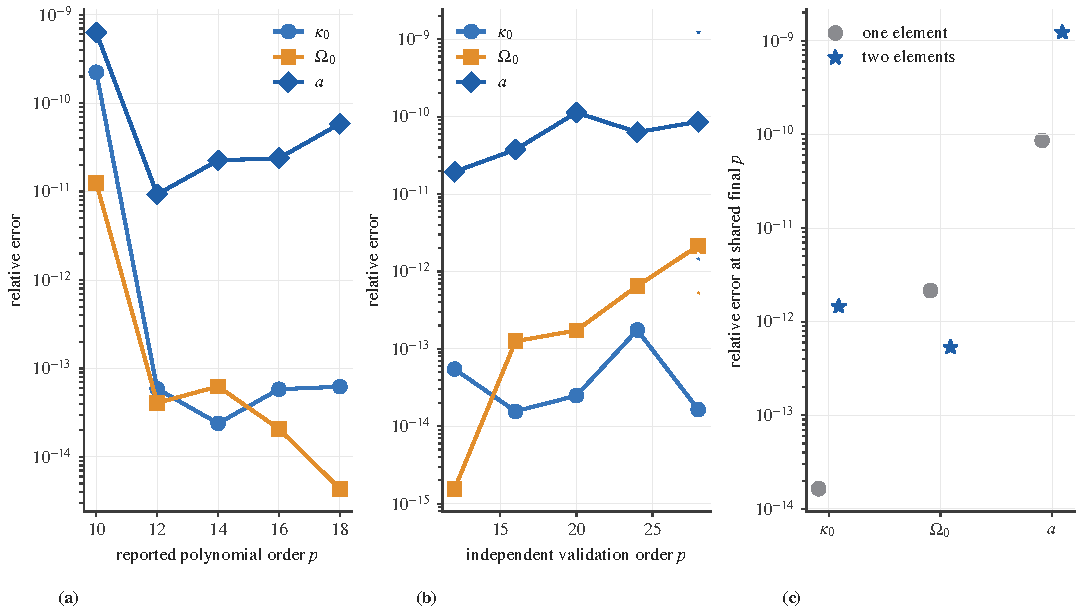
\includegraphics[width=\textwidth]{../figures/supplementary/figure_s01_polynomial_two_element.pdf}
  \caption{\SupplementaryFigureOneCaption}
  \label{fig:supplement-01}
\end{figure}

\begin{figure}[p]
  \centering
  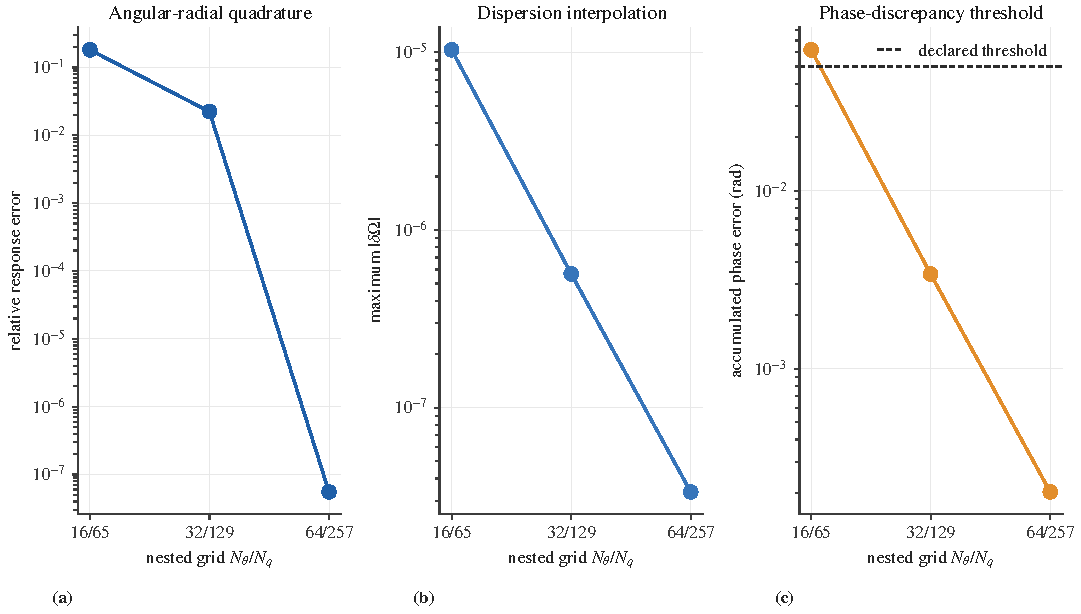
\includegraphics[width=\textwidth]{../figures/supplementary/figure_s02_quadrature_phase.pdf}
  \caption{\SupplementaryFigureTwoCaption}
  \label{fig:supplement-02}
\end{figure}

\begin{figure}[p]
  \centering
  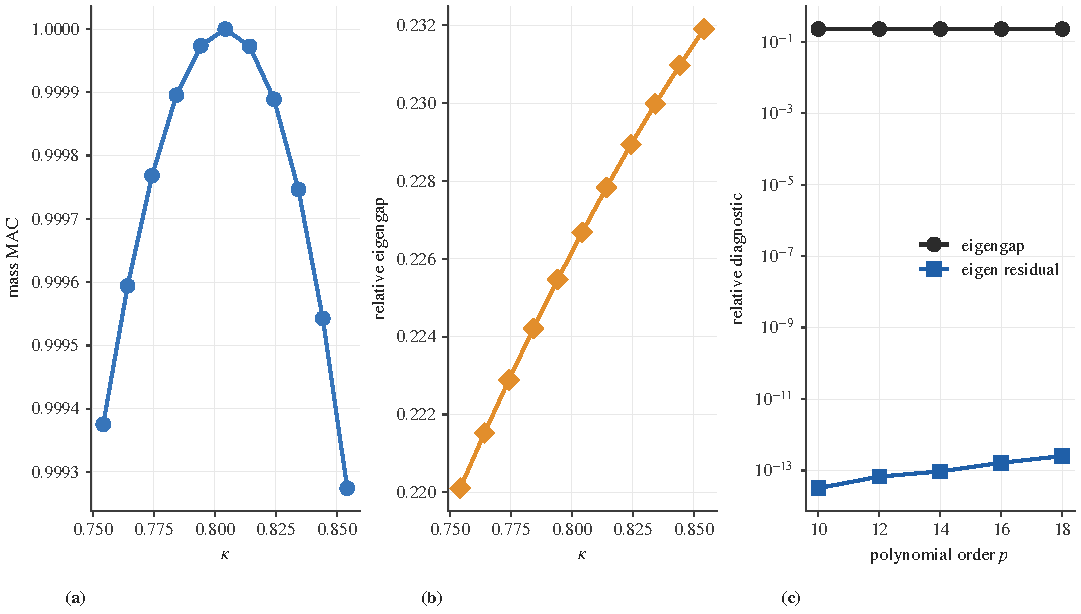
\includegraphics[width=\textwidth]{../figures/supplementary/figure_s03_mode_tracking.pdf}
  \caption{\SupplementaryFigureThreeCaption}
  \label{fig:supplement-03}
\end{figure}

\begin{figure}[p]
  \centering
  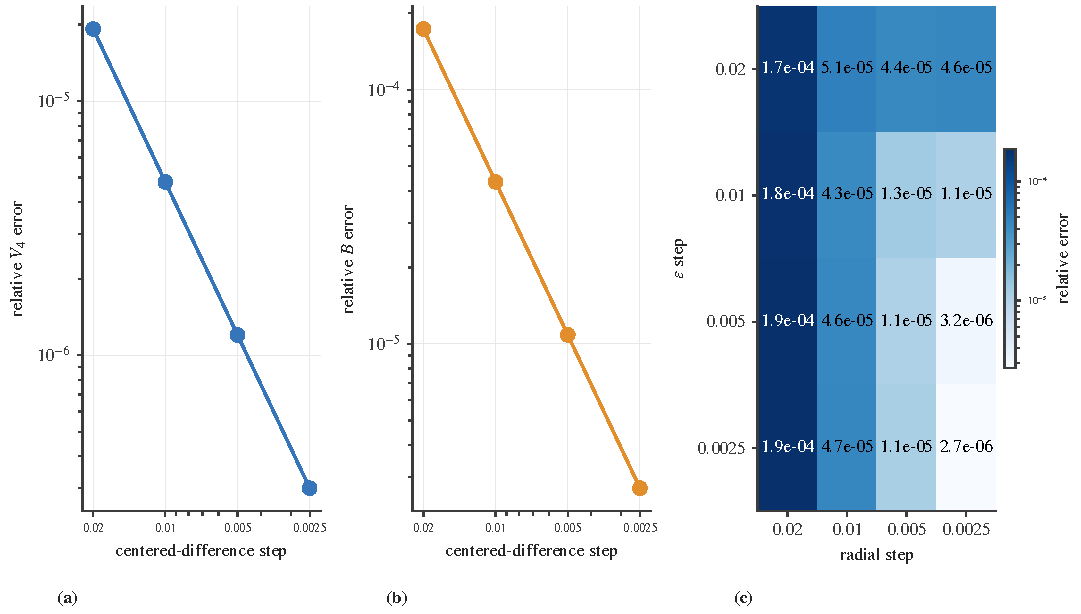
\includegraphics[width=\textwidth]{../figures/supplementary/figure_s04_fd_convergence.pdf}
  \caption{\SupplementaryFigureFourCaption}
  \label{fig:supplement-04}
\end{figure}

\begin{figure}[p]
  \centering
  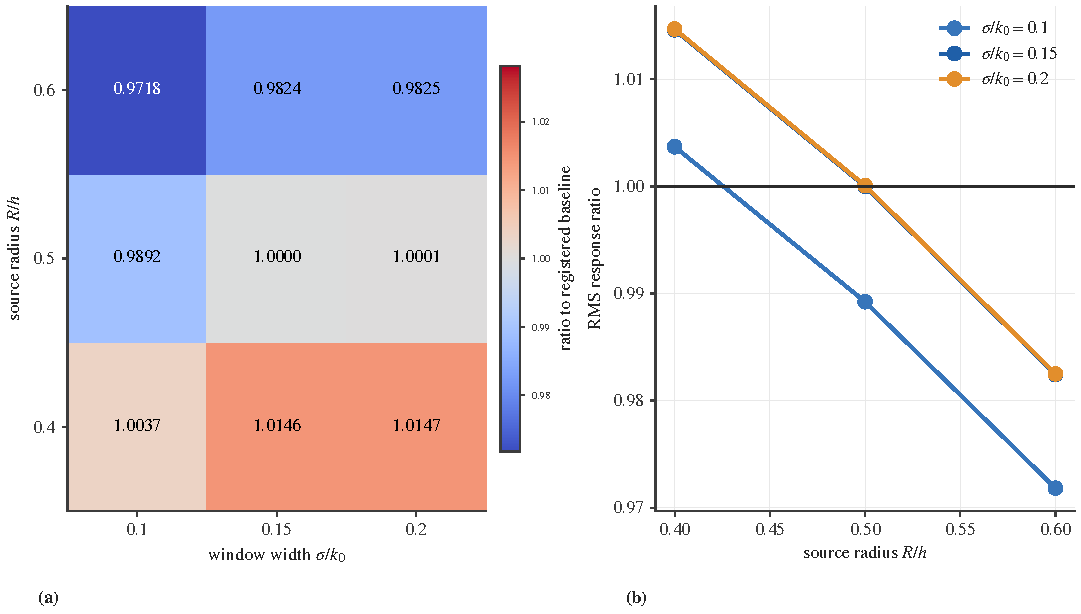
\includegraphics[width=\textwidth]{../figures/supplementary/figure_s05_source_window_sensitivity.pdf}
  \caption{\SupplementaryFigureFiveCaption}
  \label{fig:supplement-05}
\end{figure}

\begin{figure}[p]
  \centering
  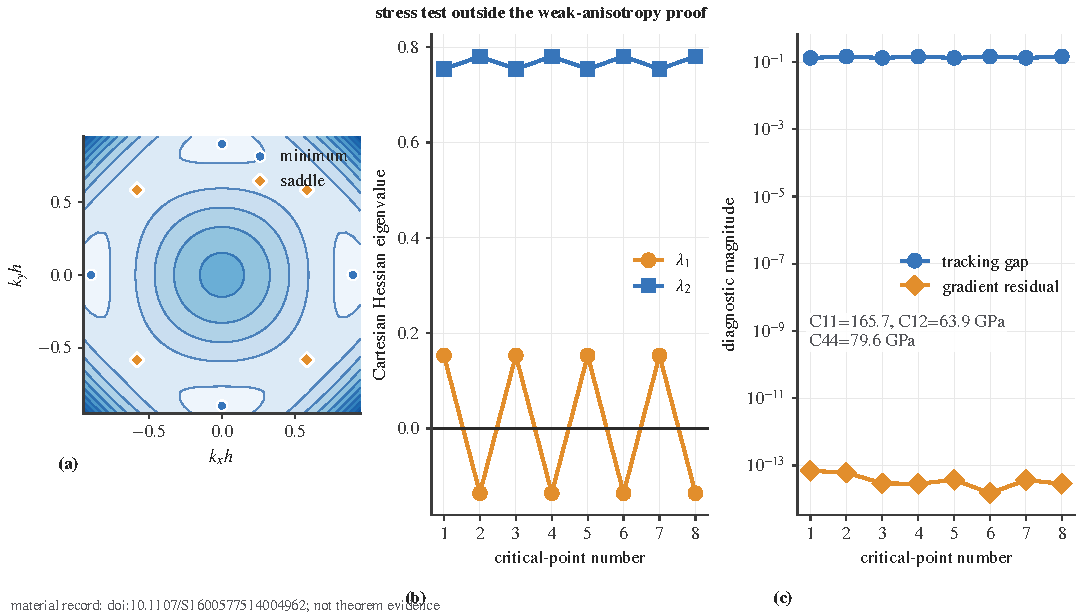
\includegraphics[width=\textwidth]{../figures/supplementary/figure_s06_silicon_stress_test.pdf}
  \caption{\SupplementaryFigureSixCaption}
  \label{fig:supplement-06}
\end{figure}

\clearpage


\end{document}
